\INEchaptercarta{Caracterización escolar de los ocupados y desocupados}{}

%
%
%
\cajita{Ocupados: educación primaria}{En el 2014, el  57.9\% de la población ocupada reportó tener algún grado del nivel primario, aprobado. Este conjunto incluye a la población que no tiene ningún nivel de escolaridad aprobado.}{Proporción de población ocupada que tiene hasta sexto grado de primaria}{República de Guatemala, serie histórica, en porcentaje}{\ \\[0mm]\begin{tikzpicture}[x=1pt,y=1pt]  % Created by tikzDevice version 0.9 on 2016-02-28 17:13:01
% !TEX encoding = UTF-8 Unicode
\definecolor{fillColor}{RGB}{255,255,255}
\path[use as bounding box,fill=fillColor,fill opacity=0.00] (0,0) rectangle (289.08,198.74);
\begin{scope}
\path[clip] (  0.00,  0.00) rectangle (289.08,198.74);

\path[] (  0.00,  0.00) rectangle (289.08,198.74);
\end{scope}
\begin{scope}
\path[clip] (  0.00,  0.00) rectangle (289.08,198.74);

\path[] ( -0.52, 15.61) rectangle (280.54,191.48);

\path[] (  0.00, 47.74) --
	(280.54, 47.74);

\path[] (  0.00, 95.99) --
	(280.54, 95.99);

\path[] (  0.00,144.25) --
	(280.54,144.25);

\path[] (  0.00, 23.61) --
	(280.54, 23.61);

\path[] (  0.00, 71.86) --
	(280.54, 71.86);

\path[] (  0.00,120.12) --
	(280.54,120.12);

\path[] (  0.00,168.38) --
	(280.54,168.38);

\path[] ( 39.63, 15.61) --
	( 39.63,191.48);

\path[] (106.55, 15.61) --
	(106.55,191.48);

\path[] (173.47, 15.61) --
	(173.47,191.48);

\path[] (240.39, 15.61) --
	(240.39,191.48);
\definecolor{drawColor}{RGB}{0,0,255}

\path[draw=drawColor,line width= 1.7pt,line join=round] ( 39.63,183.49) --
	(106.55,173.58) --
	(173.47,170.79) --
	(240.39,163.42);
\definecolor{drawColor}{RGB}{0,0,0}

\node[text=drawColor,anchor=base,inner sep=0pt, outer sep=0pt, scale=  1.02] at ( 39.63,187.46) {66.3};

\node[text=drawColor,anchor=base west,inner sep=0pt, outer sep=0pt, scale=  1.02] at (106.55,177.55) {62.2};

\node[text=drawColor,anchor=base west,inner sep=0pt, outer sep=0pt, scale=  1.02] at (173.47,174.76) {61.0};

\node[text=drawColor,anchor=base,inner sep=0pt, outer sep=0pt, scale=  1.02] at (240.39,151.51) {57.9};

\path[draw=drawColor,line width= 0.1pt,line join=round] (  0.00, 23.61) -- (280.54, 23.61);

\path[] ( -0.52, 15.61) rectangle (280.54,191.48);
\end{scope}
\begin{scope}
\path[clip] (  0.00,  0.00) rectangle (289.08,198.74);

\path[] (  0.00, 15.61) --
	(280.54, 15.61);
\end{scope}
\begin{scope}
\path[clip] (  0.00,  0.00) rectangle (289.08,198.74);

\path[] ( 39.63, 12.86) --
	( 39.63, 15.61);

\path[] (106.55, 12.86) --
	(106.55, 15.61);

\path[] (173.47, 12.86) --
	(173.47, 15.61);

\path[] (240.39, 12.86) --
	(240.39, 15.61);
\end{scope}
\begin{scope}
\path[clip] (  0.00,  0.00) rectangle (289.08,198.74);
\definecolor{drawColor}{RGB}{0,0,0}

\node[text=drawColor,anchor=base,inner sep=0pt, outer sep=0pt, scale=  1.00] at ( 39.63,  2.85) {2011};

\node[text=drawColor,anchor=base,inner sep=0pt, outer sep=0pt, scale=  1.00] at (106.55,  2.85) {2012};

\node[text=drawColor,anchor=base,inner sep=0pt, outer sep=0pt, scale=  1.00] at (173.47,  2.85) {2013};

\node[text=drawColor,anchor=base,inner sep=0pt, outer sep=0pt, scale=  1.00] at (240.39,  2.85) {2014};
\end{scope}
  \end{tikzpicture} }{Instituto Nacional de Estadística, con datos de ENEI II-2014}


\cajita{Ocupados: educación primaria y la rama de actividad}{Según la rama de actividad del lugar donde labora la población ocupada, el 87.1\% de las personas que laboran en empresas dedicadas a la agricultura tienen aprobado, a lo sumo, sexto primaria.
	
	 Por otro lado, el 6.3\% de las personas ocupadas que laboran en empresas dedicadas a comunicaciones tienen a lo sumo aprobado sexto primaria.}{Proporción de población ocupada que tiene hasta sexto grado de primaria por rama de actividad}{República de Guatemala, año 2014, en porcentaje}{\ \\[0mm]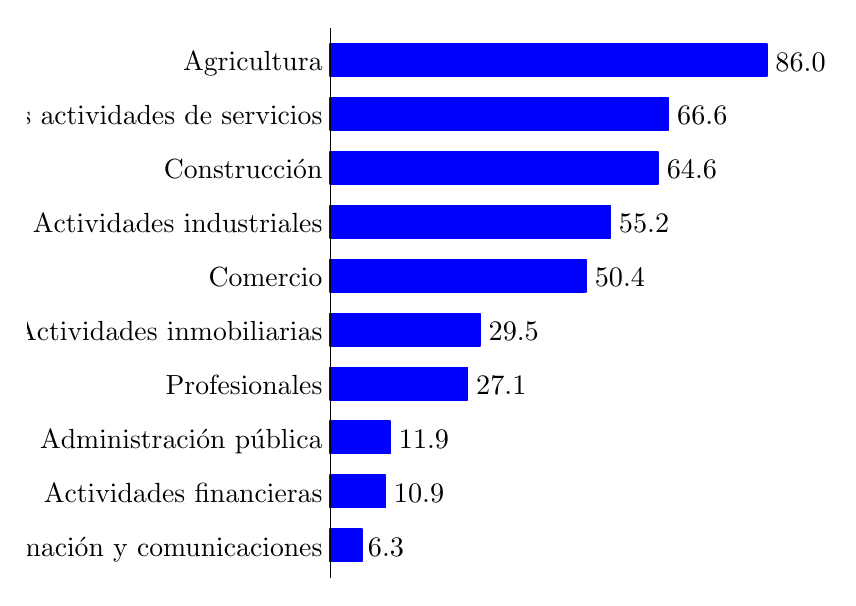
\begin{tikzpicture}[x=1pt,y=1pt]  % Created by tikzDevice version 0.9 on 2016-02-28 20:01:55
% !TEX encoding = UTF-8 Unicode
\definecolor{fillColor}{RGB}{255,255,255}
\path[use as bounding box,fill=fillColor,fill opacity=0.00] (0,0) rectangle (289.08,198.74);
\begin{scope}
\path[clip] (  0.00,  0.00) rectangle (289.08,198.74);

\path[] (  0.00,  0.00) rectangle (289.08,198.74);
\end{scope}
\begin{scope}
\path[clip] (  0.00,  0.00) rectangle (289.08,198.74);

\path[] (109.26,  0.00) rectangle (267.09,198.74);

\path[] (109.26, 11.69) --
	(267.09, 11.69);

\path[] (109.26, 31.18) --
	(267.09, 31.18);

\path[] (109.26, 50.66) --
	(267.09, 50.66);

\path[] (109.26, 70.14) --
	(267.09, 70.14);

\path[] (109.26, 89.63) --
	(267.09, 89.63);

\path[] (109.26,109.11) --
	(267.09,109.11);

\path[] (109.26,128.60) --
	(267.09,128.60);

\path[] (109.26,148.08) --
	(267.09,148.08);

\path[] (109.26,167.57) --
	(267.09,167.57);

\path[] (109.26,187.05) --
	(267.09,187.05);
\definecolor{drawColor}{RGB}{0,0,255}
\definecolor{fillColor}{RGB}{0,0,255}

\path[draw=drawColor,line width= 0.6pt,line join=round,fill=fillColor] (109.26,  5.85) rectangle (120.73, 17.54);

\path[draw=drawColor,line width= 0.6pt,line join=round,fill=fillColor] (109.26, 25.33) rectangle (129.25, 37.02);

\path[draw=drawColor,line width= 0.6pt,line join=round,fill=fillColor] (109.26, 44.81) rectangle (131.02, 56.51);

\path[draw=drawColor,line width= 0.6pt,line join=round,fill=fillColor] (109.26, 64.30) rectangle (158.94, 75.99);

\path[draw=drawColor,line width= 0.6pt,line join=round,fill=fillColor] (109.26, 83.78) rectangle (163.45, 95.47);

\path[draw=drawColor,line width= 0.6pt,line join=round,fill=fillColor] (109.26,103.27) rectangle (201.80,114.96);

\path[draw=drawColor,line width= 0.6pt,line join=round,fill=fillColor] (109.26,122.75) rectangle (210.55,134.44);

\path[draw=drawColor,line width= 0.6pt,line join=round,fill=fillColor] (109.26,142.24) rectangle (227.82,153.93);

\path[draw=drawColor,line width= 0.6pt,line join=round,fill=fillColor] (109.26,161.72) rectangle (231.57,173.41);

\path[draw=drawColor,line width= 0.6pt,line join=round,fill=fillColor] (109.26,181.21) rectangle (267.09,192.90);
\definecolor{drawColor}{RGB}{0,0,0}

\path[draw=drawColor,line width= 0.1pt,line join=round] (109.26,  0.00) -- (109.26,198.74);

\node[text=drawColor,anchor=base west,inner sep=0pt, outer sep=0pt, scale=  1.02] at (122.97,  7.72) {6.3};

\node[text=drawColor,anchor=base west,inner sep=0pt, outer sep=0pt, scale=  1.02] at (132.37, 27.20) {10.9};

\node[text=drawColor,anchor=base west,inner sep=0pt, outer sep=0pt, scale=  1.02] at (134.15, 46.69) {11.9};

\node[text=drawColor,anchor=base west,inner sep=0pt, outer sep=0pt, scale=  1.02] at (162.07, 66.17) {27.1};

\node[text=drawColor,anchor=base west,inner sep=0pt, outer sep=0pt, scale=  1.02] at (166.58, 85.66) {29.5};

\node[text=drawColor,anchor=base west,inner sep=0pt, outer sep=0pt, scale=  1.02] at (204.93,105.14) {50.4};

\node[text=drawColor,anchor=base west,inner sep=0pt, outer sep=0pt, scale=  1.02] at (213.67,124.63) {55.2};

\node[text=drawColor,anchor=base west,inner sep=0pt, outer sep=0pt, scale=  1.02] at (230.95,144.11) {64.6};

\node[text=drawColor,anchor=base west,inner sep=0pt, outer sep=0pt, scale=  1.02] at (234.70,163.60) {66.6};

\node[text=drawColor,anchor=base west,inner sep=0pt, outer sep=0pt, scale=  1.02] at (270.21,183.08) {86.0};

\path[] (109.26,  0.00) rectangle (267.09,198.74);
\end{scope}
\begin{scope}
\path[clip] (  0.00,  0.00) rectangle (289.08,198.74);

\path[] (109.26,  0.00) --
	(109.26,198.74);
\end{scope}
\begin{scope}
\path[clip] (  0.00,  0.00) rectangle (289.08,198.74);
\definecolor{drawColor}{RGB}{0,0,0}

\node[text=drawColor,anchor=base east,inner sep=0pt, outer sep=0pt, scale=  1.00] at (106.51,  7.78) {Información y comunicaciones};

\node[text=drawColor,anchor=base east,inner sep=0pt, outer sep=0pt, scale=  1.00] at (106.51, 27.27) {Actividades financieras };

\node[text=drawColor,anchor=base east,inner sep=0pt, outer sep=0pt, scale=  1.00] at (106.51, 46.75) {Administración pública };

\node[text=drawColor,anchor=base east,inner sep=0pt, outer sep=0pt, scale=  1.00] at (106.51, 66.24) {Profesionales};

\node[text=drawColor,anchor=base east,inner sep=0pt, outer sep=0pt, scale=  1.00] at (106.51, 85.72) {Actividades inmobiliarias};

\node[text=drawColor,anchor=base east,inner sep=0pt, outer sep=0pt, scale=  1.00] at (106.51,105.21) {Comercio };

\node[text=drawColor,anchor=base east,inner sep=0pt, outer sep=0pt, scale=  1.00] at (106.51,124.69) {Actividades  industriales};

\node[text=drawColor,anchor=base east,inner sep=0pt, outer sep=0pt, scale=  1.00] at (106.51,144.17) {Construcción};

\node[text=drawColor,anchor=base east,inner sep=0pt, outer sep=0pt, scale=  1.00] at (106.51,163.66) {Otras actividades de servicios};

\node[text=drawColor,anchor=base east,inner sep=0pt, outer sep=0pt, scale=  1.00] at (106.51,183.14) {Agricultura};
\end{scope}
\begin{scope}
\path[clip] (  0.00,  0.00) rectangle (289.08,198.74);

\path[] (106.51, 11.69) --
	(109.26, 11.69);

\path[] (106.51, 31.18) --
	(109.26, 31.18);

\path[] (106.51, 50.66) --
	(109.26, 50.66);

\path[] (106.51, 70.14) --
	(109.26, 70.14);

\path[] (106.51, 89.63) --
	(109.26, 89.63);

\path[] (106.51,109.11) --
	(109.26,109.11);

\path[] (106.51,128.60) --
	(109.26,128.60);

\path[] (106.51,148.08) --
	(109.26,148.08);

\path[] (106.51,167.57) --
	(109.26,167.57);

\path[] (106.51,187.05) --
	(109.26,187.05);
\end{scope}
  \end{tikzpicture} }{Instituto Nacional de Estadística, con datos de ENEI II-2014}

%

\cajita{Ocupados: educación primaria y la ocupación}{Según la categoría ocupacional de las población ocupada, el 84.7\% de los agricultores tiene aprobado a lo sumo sexto primaria, así mismo el 81.2\% de las población cuya ocupación está clasificada como ocupaciones elementales su formación está entre ninguna y sexto primaria. }{Proporción de población ocupada que tiene hasta sexto grado de primaria por categoría ocupacional}{República de Guatemala, año 2014, en porcentaje}{\ \\[0mm]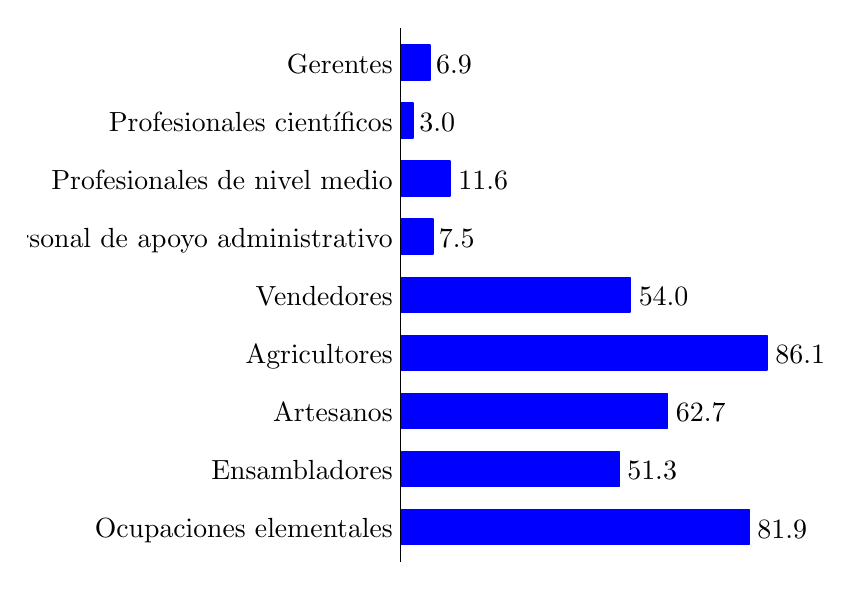
\begin{tikzpicture}[x=1pt,y=1pt]  % Created by tikzDevice version 0.9 on 2015-12-11 10:47:45
% !TEX encoding = UTF-8 Unicode
\definecolor{fillColor}{RGB}{255,255,255}
\path[use as bounding box,fill=fillColor,fill opacity=0.00] (0,0) rectangle (289.08,198.74);
\begin{scope}
\path[clip] (  0.00,  0.00) rectangle (289.08,198.74);

\path[] (  0.00,  0.00) rectangle (289.08,198.74);
\end{scope}
\begin{scope}
\path[clip] (  0.00,  0.00) rectangle (289.08,198.74);

\path[] (134.76,  5.69) rectangle (267.09,198.74);

\path[] (134.76, 18.28) --
	(267.09, 18.28);

\path[] (134.76, 39.26) --
	(267.09, 39.26);

\path[] (134.76, 60.25) --
	(267.09, 60.25);

\path[] (134.76, 81.23) --
	(267.09, 81.23);

\path[] (134.76,102.22) --
	(267.09,102.22);

\path[] (134.76,123.20) --
	(267.09,123.20);

\path[] (134.76,144.18) --
	(267.09,144.18);

\path[] (134.76,165.17) --
	(267.09,165.17);

\path[] (134.76,186.15) --
	(267.09,186.15);
\definecolor{drawColor}{RGB}{0,0,255}
\definecolor{fillColor}{RGB}{0,0,255}

\path[draw=drawColor,line width= 0.6pt,line join=round,fill=fillColor] (134.76, 11.99) rectangle (260.56, 24.58);

\path[draw=drawColor,line width= 0.6pt,line join=round,fill=fillColor] (134.76, 32.97) rectangle (213.56, 45.56);

\path[draw=drawColor,line width= 0.6pt,line join=round,fill=fillColor] (134.76, 53.95) rectangle (231.08, 66.54);

\path[draw=drawColor,line width= 0.6pt,line join=round,fill=fillColor] (134.76, 74.94) rectangle (267.09, 87.53);

\path[draw=drawColor,line width= 0.6pt,line join=round,fill=fillColor] (134.76, 95.92) rectangle (217.70,108.51);

\path[draw=drawColor,line width= 0.6pt,line join=round,fill=fillColor] (134.76,116.91) rectangle (146.35,129.50);

\path[draw=drawColor,line width= 0.6pt,line join=round,fill=fillColor] (134.76,137.89) rectangle (152.51,150.48);

\path[draw=drawColor,line width= 0.6pt,line join=round,fill=fillColor] (134.76,158.87) rectangle (139.35,171.46);

\path[draw=drawColor,line width= 0.6pt,line join=round,fill=fillColor] (134.76,179.86) rectangle (145.40,192.45);
\definecolor{drawColor}{RGB}{0,0,0}

\path[draw=drawColor,line width= 0.1pt,line join=round] (134.76,  5.69) -- (134.76,198.74);

\node[text=drawColor,anchor=base west,inner sep=0pt, outer sep=0pt, scale=  1.01] at (263.68, 14.32) {81.9};

\node[text=drawColor,anchor=base west,inner sep=0pt, outer sep=0pt, scale=  1.01] at (216.67, 35.31) {51.3};

\node[text=drawColor,anchor=base west,inner sep=0pt, outer sep=0pt, scale=  1.01] at (234.20, 56.29) {62.7};

\node[text=drawColor,anchor=base west,inner sep=0pt, outer sep=0pt, scale=  1.01] at (270.20, 77.28) {86.1};

\node[text=drawColor,anchor=base west,inner sep=0pt, outer sep=0pt, scale=  1.01] at (220.82, 98.26) {54.0};

\node[text=drawColor,anchor=base west,inner sep=0pt, outer sep=0pt, scale=  1.01] at (148.58,119.24) {7.5};

\node[text=drawColor,anchor=base west,inner sep=0pt, outer sep=0pt, scale=  1.01] at (155.63,140.23) {11.6};

\node[text=drawColor,anchor=base west,inner sep=0pt, outer sep=0pt, scale=  1.01] at (141.58,161.21) {3.0};

\node[text=drawColor,anchor=base west,inner sep=0pt, outer sep=0pt, scale=  1.01] at (147.63,182.20) {6.9};

\path[] (134.76,  5.69) rectangle (267.09,198.74);
\end{scope}
\begin{scope}
\path[clip] (  0.00,  0.00) rectangle (289.08,198.74);

\path[] (134.76,  5.69) --
	(134.76,198.74);
\end{scope}
\begin{scope}
\path[clip] (  0.00,  0.00) rectangle (289.08,198.74);
\definecolor{drawColor}{RGB}{0,0,0}

\node[text=drawColor,anchor=base east,inner sep=0pt, outer sep=0pt, scale=  1.00] at (131.91, 14.37) {Ocupaciones elementales};

\node[text=drawColor,anchor=base east,inner sep=0pt, outer sep=0pt, scale=  1.00] at (131.91, 35.36) {Ensambladores};

\node[text=drawColor,anchor=base east,inner sep=0pt, outer sep=0pt, scale=  1.00] at (131.91, 56.34) {Artesanos};

\node[text=drawColor,anchor=base east,inner sep=0pt, outer sep=0pt, scale=  1.00] at (131.91, 77.32) {Agricultores};

\node[text=drawColor,anchor=base east,inner sep=0pt, outer sep=0pt, scale=  1.00] at (131.91, 98.31) {Vendedores};

\node[text=drawColor,anchor=base east,inner sep=0pt, outer sep=0pt, scale=  1.00] at (131.91,119.29) {Personal de apoyo administrativo};

\node[text=drawColor,anchor=base east,inner sep=0pt, outer sep=0pt, scale=  1.00] at (131.91,140.28) {Profesionales de nivel medio};

\node[text=drawColor,anchor=base east,inner sep=0pt, outer sep=0pt, scale=  1.00] at (131.91,161.26) {Profesionales científicos};

\node[text=drawColor,anchor=base east,inner sep=0pt, outer sep=0pt, scale=  1.00] at (131.91,182.24) {Gerentes};
\end{scope}
\begin{scope}
\path[clip] (  0.00,  0.00) rectangle (289.08,198.74);

\path[] (131.91, 18.28) --
	(136.18, 18.28);

\path[] (131.91, 39.26) --
	(136.18, 39.26);

\path[] (131.91, 60.25) --
	(136.18, 60.25);

\path[] (131.91, 81.23) --
	(136.18, 81.23);

\path[] (131.91,102.22) --
	(136.18,102.22);

\path[] (131.91,123.20) --
	(136.18,123.20);

\path[] (131.91,144.18) --
	(136.18,144.18);

\path[] (131.91,165.17) --
	(136.18,165.17);

\path[] (131.91,186.15) --
	(136.18,186.15);
\end{scope}
\begin{scope}
\path[clip] (  0.00,  0.00) rectangle (289.08,198.74);

\path[] (134.76,  5.69) --
	(267.09,  5.69);
\end{scope}
  \end{tikzpicture} }{Instituto Nacional de Estadística, con datos de ENEI II-2014}


\cajita{Ocupados: IGSS y escolaridad}{Según el nivel de escolaridad de la población ocupada, el 59.8\% de quienes  que reportan tener educación superior están afiliados al IGSS.
	
	Asimismo, de la población sin ningún nivel de escolaridad aprobado, el 2.7\% está afiliado al IGSS.}{Proporción de la población ocupada que es afiliado activo del IGSS, según nivel de escolaridad}{República de Guatemala, año 2014, en porcentaje}{\ \\[0mm]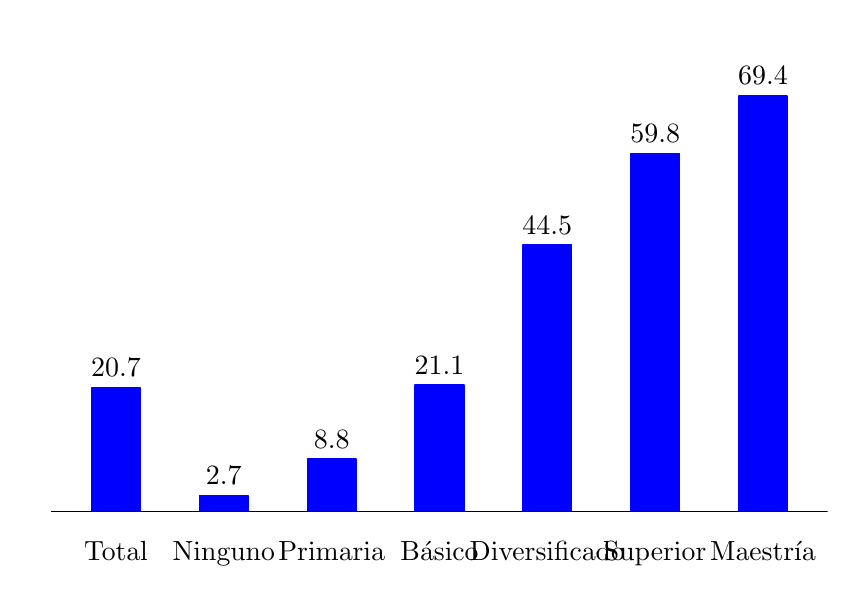
\begin{tikzpicture}[x=1pt,y=1pt]  % Created by tikzDevice version 0.9 on 2015-12-11 10:47:45
% !TEX encoding = UTF-8 Unicode
\definecolor{fillColor}{RGB}{255,255,255}
\path[use as bounding box,fill=fillColor,fill opacity=0.00] (0,0) rectangle (289.08,198.74);
\begin{scope}
\path[clip] (  0.00,  0.00) rectangle (289.08,198.74);

\path[] (  0.00,  0.00) rectangle (289.08,198.74);
\end{scope}
\begin{scope}
\path[clip] (  0.00,  0.00) rectangle (289.08,198.74);

\path[] (  8.54, 16.35) rectangle (289.08,181.67);

\path[] ( 31.91, 16.35) --
	( 31.91,181.67);

\path[] ( 70.88, 16.35) --
	( 70.88,181.67);

\path[] (109.84, 16.35) --
	(109.84,181.67);

\path[] (148.81, 16.35) --
	(148.81,181.67);

\path[] (187.77, 16.35) --
	(187.77,181.67);

\path[] (226.74, 16.35) --
	(226.74,181.67);

\path[] (265.70, 16.35) --
	(265.70,181.67);
\definecolor{drawColor}{RGB}{0,0,255}
\definecolor{fillColor}{RGB}{0,0,255}

\path[draw=drawColor,line width= 0.6pt,line join=round,fill=fillColor] ( 23.15, 23.87) rectangle ( 40.68, 68.73);

\path[draw=drawColor,line width= 0.6pt,line join=round,fill=fillColor] ( 62.11, 23.87) rectangle ( 79.65, 29.74);

\path[draw=drawColor,line width= 0.6pt,line join=round,fill=fillColor] (101.08, 23.87) rectangle (118.61, 42.88);

\path[draw=drawColor,line width= 0.6pt,line join=round,fill=fillColor] (140.04, 23.87) rectangle (157.57, 69.53);

\path[draw=drawColor,line width= 0.6pt,line join=round,fill=fillColor] (179.01, 23.87) rectangle (196.54,120.19);

\path[draw=drawColor,line width= 0.6pt,line join=round,fill=fillColor] (217.97, 23.87) rectangle (235.50,153.29);

\path[draw=drawColor,line width= 0.6pt,line join=round,fill=fillColor] (256.93, 23.87) rectangle (274.47,174.16);
\definecolor{drawColor}{RGB}{0,0,0}

\path[draw=drawColor,line width= 0.1pt,line join=round] (  8.54, 23.87) -- (289.08, 23.87);

\node[text=drawColor,anchor=base,inner sep=0pt, outer sep=0pt, scale=  1.01] at ( 31.91, 72.68) {20.7};

\node[text=drawColor,anchor=base,inner sep=0pt, outer sep=0pt, scale=  1.01] at ( 70.88, 33.70) {2.7};

\node[text=drawColor,anchor=base,inner sep=0pt, outer sep=0pt, scale=  1.01] at (109.84, 46.84) {8.8};

\node[text=drawColor,anchor=base,inner sep=0pt, outer sep=0pt, scale=  1.01] at (148.81, 73.49) {21.1};

\node[text=drawColor,anchor=base,inner sep=0pt, outer sep=0pt, scale=  1.01] at (187.77,124.14) {44.5};

\node[text=drawColor,anchor=base,inner sep=0pt, outer sep=0pt, scale=  1.01] at (226.74,157.24) {59.8};

\node[text=drawColor,anchor=base,inner sep=0pt, outer sep=0pt, scale=  1.01] at (265.70,178.11) {69.4};

\path[] (  8.54, 16.35) rectangle (289.08,181.67);
\end{scope}
\begin{scope}
\path[clip] (  0.00,  0.00) rectangle (289.08,198.74);

\path[] (  8.54, 16.35) --
	(  8.54,181.67);
\end{scope}
\begin{scope}
\path[clip] (  0.00,  0.00) rectangle (289.08,198.74);

\path[] (  8.54, 16.35) --
	(289.08, 16.35);
\end{scope}
\begin{scope}
\path[clip] (  0.00,  0.00) rectangle (289.08,198.74);

\path[] ( 31.91, 12.08) --
	( 31.91, 16.35);

\path[] ( 70.88, 12.08) --
	( 70.88, 16.35);

\path[] (109.84, 12.08) --
	(109.84, 16.35);

\path[] (148.81, 12.08) --
	(148.81, 16.35);

\path[] (187.77, 12.08) --
	(187.77, 16.35);

\path[] (226.74, 12.08) --
	(226.74, 16.35);

\path[] (265.70, 12.08) --
	(265.70, 16.35);
\end{scope}
\begin{scope}
\path[clip] (  0.00,  0.00) rectangle (289.08,198.74);
\definecolor{drawColor}{RGB}{0,0,0}

\node[text=drawColor,anchor=base,inner sep=0pt, outer sep=0pt, scale=  1.00] at ( 31.91,  6.04) {Total};

\node[text=drawColor,anchor=base,inner sep=0pt, outer sep=0pt, scale=  1.00] at ( 70.88,  6.04) {Ninguno};

\node[text=drawColor,anchor=base,inner sep=0pt, outer sep=0pt, scale=  1.00] at (109.84,  6.04) {Primaria};

\node[text=drawColor,anchor=base,inner sep=0pt, outer sep=0pt, scale=  1.00] at (148.81,  6.04) {Básico};

\node[text=drawColor,anchor=base,inner sep=0pt, outer sep=0pt, scale=  1.00] at (187.77,  6.04) {Diversificado};

\node[text=drawColor,anchor=base,inner sep=0pt, outer sep=0pt, scale=  1.00] at (226.74,  6.04) {Superior};

\node[text=drawColor,anchor=base,inner sep=0pt, outer sep=0pt, scale=  1.00] at (265.70,  6.04) {Maestría};
\end{scope}
  \end{tikzpicture} }{Instituto Nacional de Estadística, con datos de ENEI II-2014}


\cajita{Ocupados: sector informal y escolaridad}{Según el nivel de escolaridad de la población ocupada, el 11.8\% de quienes  que reportan tener educación superior están laborando en el sector informal.
	
	 Asimismo, de la población sin ningún nivel de escolaridad aprobado, el 92.9\% trabaja en ese sector.}{Proporción de la población ocupada que labora en el sector informal según nivel de escolaridad}{República de Guatemala, año 2014, en porcentaje}{\ \\[0mm]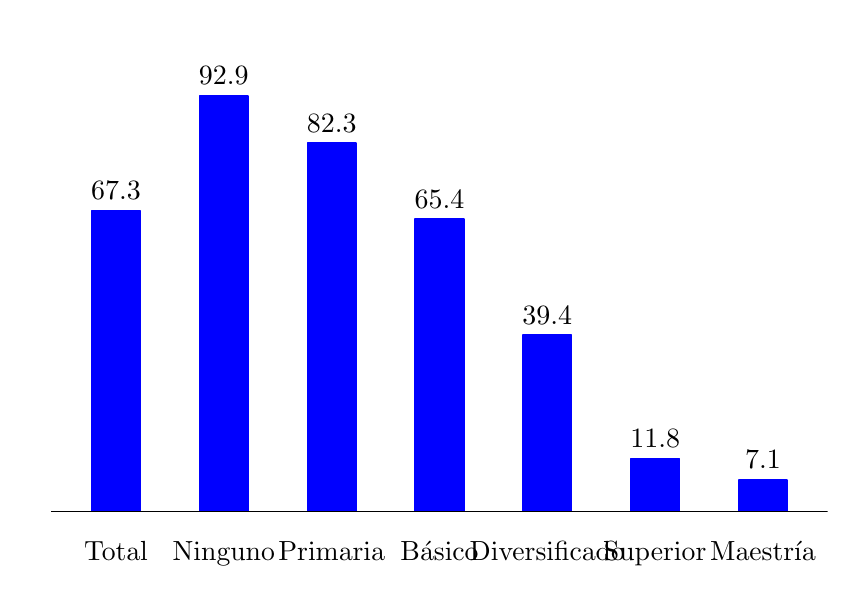
\begin{tikzpicture}[x=1pt,y=1pt]  % Created by tikzDevice version 0.9 on 2015-12-11 10:47:46
% !TEX encoding = UTF-8 Unicode
\definecolor{fillColor}{RGB}{255,255,255}
\path[use as bounding box,fill=fillColor,fill opacity=0.00] (0,0) rectangle (289.08,198.74);
\begin{scope}
\path[clip] (  0.00,  0.00) rectangle (289.08,198.74);

\path[] (  0.00,  0.00) rectangle (289.08,198.74);
\end{scope}
\begin{scope}
\path[clip] (  0.00,  0.00) rectangle (289.08,198.74);

\path[] (  8.54, 16.35) rectangle (289.08,181.67);

\path[] ( 31.91, 16.35) --
	( 31.91,181.67);

\path[] ( 70.88, 16.35) --
	( 70.88,181.67);

\path[] (109.84, 16.35) --
	(109.84,181.67);

\path[] (148.81, 16.35) --
	(148.81,181.67);

\path[] (187.77, 16.35) --
	(187.77,181.67);

\path[] (226.74, 16.35) --
	(226.74,181.67);

\path[] (265.70, 16.35) --
	(265.70,181.67);
\definecolor{drawColor}{RGB}{0,0,255}
\definecolor{fillColor}{RGB}{0,0,255}

\path[draw=drawColor,line width= 0.6pt,line join=round,fill=fillColor] ( 23.15, 23.87) rectangle ( 40.68,132.65);

\path[draw=drawColor,line width= 0.6pt,line join=round,fill=fillColor] ( 62.11, 23.87) rectangle ( 79.65,174.16);

\path[draw=drawColor,line width= 0.6pt,line join=round,fill=fillColor] (101.08, 23.87) rectangle (118.61,157.06);

\path[draw=drawColor,line width= 0.6pt,line join=round,fill=fillColor] (140.04, 23.87) rectangle (157.57,129.59);

\path[draw=drawColor,line width= 0.6pt,line join=round,fill=fillColor] (179.01, 23.87) rectangle (196.54, 87.65);

\path[draw=drawColor,line width= 0.6pt,line join=round,fill=fillColor] (217.97, 23.87) rectangle (235.50, 43.02);

\path[draw=drawColor,line width= 0.6pt,line join=round,fill=fillColor] (256.93, 23.87) rectangle (274.47, 35.35);
\definecolor{drawColor}{RGB}{0,0,0}

\path[draw=drawColor,line width= 0.1pt,line join=round] (  8.54, 23.87) -- (289.08, 23.87);

\node[text=drawColor,anchor=base,inner sep=0pt, outer sep=0pt, scale=  1.01] at ( 31.91,136.61) {67.3};

\node[text=drawColor,anchor=base,inner sep=0pt, outer sep=0pt, scale=  1.01] at ( 70.88,178.11) {92.9};

\node[text=drawColor,anchor=base,inner sep=0pt, outer sep=0pt, scale=  1.01] at (109.84,161.02) {82.3};

\node[text=drawColor,anchor=base,inner sep=0pt, outer sep=0pt, scale=  1.01] at (148.81,133.55) {65.4};

\node[text=drawColor,anchor=base,inner sep=0pt, outer sep=0pt, scale=  1.01] at (187.77, 91.61) {39.4};

\node[text=drawColor,anchor=base,inner sep=0pt, outer sep=0pt, scale=  1.01] at (226.74, 46.97) {11.8};

\node[text=drawColor,anchor=base,inner sep=0pt, outer sep=0pt, scale=  1.01] at (265.70, 39.30) {7.1};

\path[] (  8.54, 16.35) rectangle (289.08,181.67);
\end{scope}
\begin{scope}
\path[clip] (  0.00,  0.00) rectangle (289.08,198.74);

\path[] (  8.54, 16.35) --
	(  8.54,181.67);
\end{scope}
\begin{scope}
\path[clip] (  0.00,  0.00) rectangle (289.08,198.74);

\path[] (  8.54, 16.35) --
	(289.08, 16.35);
\end{scope}
\begin{scope}
\path[clip] (  0.00,  0.00) rectangle (289.08,198.74);

\path[] ( 31.91, 12.08) --
	( 31.91, 16.35);

\path[] ( 70.88, 12.08) --
	( 70.88, 16.35);

\path[] (109.84, 12.08) --
	(109.84, 16.35);

\path[] (148.81, 12.08) --
	(148.81, 16.35);

\path[] (187.77, 12.08) --
	(187.77, 16.35);

\path[] (226.74, 12.08) --
	(226.74, 16.35);

\path[] (265.70, 12.08) --
	(265.70, 16.35);
\end{scope}
\begin{scope}
\path[clip] (  0.00,  0.00) rectangle (289.08,198.74);
\definecolor{drawColor}{RGB}{0,0,0}

\node[text=drawColor,anchor=base,inner sep=0pt, outer sep=0pt, scale=  1.00] at ( 31.91,  6.04) {Total};

\node[text=drawColor,anchor=base,inner sep=0pt, outer sep=0pt, scale=  1.00] at ( 70.88,  6.04) {Ninguno};

\node[text=drawColor,anchor=base,inner sep=0pt, outer sep=0pt, scale=  1.00] at (109.84,  6.04) {Primaria};

\node[text=drawColor,anchor=base,inner sep=0pt, outer sep=0pt, scale=  1.00] at (148.81,  6.04) {Básico};

\node[text=drawColor,anchor=base,inner sep=0pt, outer sep=0pt, scale=  1.00] at (187.77,  6.04) {Diversificado};

\node[text=drawColor,anchor=base,inner sep=0pt, outer sep=0pt, scale=  1.00] at (226.74,  6.04) {Superior};

\node[text=drawColor,anchor=base,inner sep=0pt, outer sep=0pt, scale=  1.00] at (265.70,  6.04) {Maestría};
\end{scope}
  \end{tikzpicture} }{Instituto Nacional de Estadística, con datos de ENEI II-2014}



\cajita{Asalariados: contratos y escolaridad}{Según el nivel de escolaridad de la población ocupada, el 83.9\% de quienes tienen educación superior cuentan con un contrato de trabajo.
	
	 Asimismo, de la población sin ningún nivel de escolaridad aprobado, el 8.4\% tiene contrato.}{Proporción de la población asalariada que  tiene contrato de trabajo, por nivel de escolaridad}{República de Guatemala, año 2014, en porcentaje}{\ \\[0mm]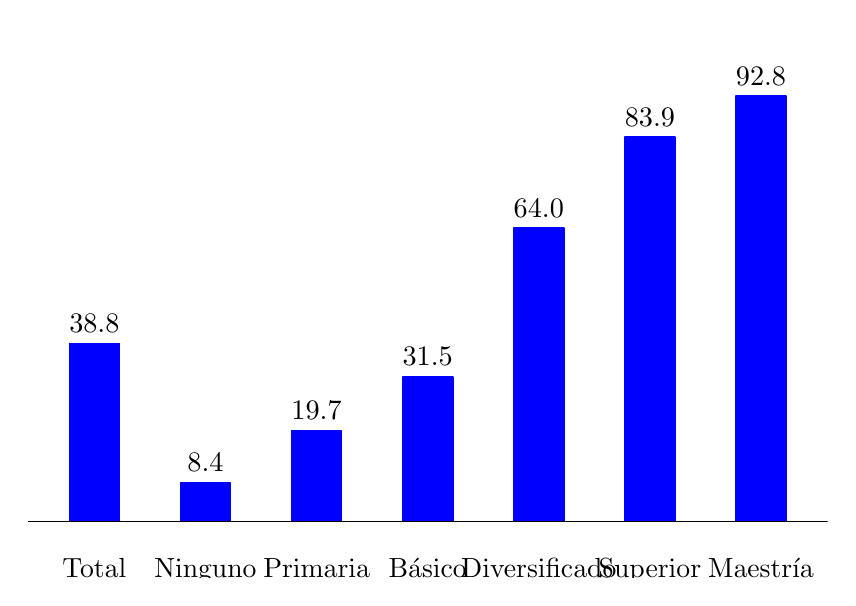
\begin{tikzpicture}[x=1pt,y=1pt]  % Created by tikzDevice version 0.9 on 2016-02-28 17:13:29
% !TEX encoding = UTF-8 Unicode
\definecolor{fillColor}{RGB}{255,255,255}
\path[use as bounding box,fill=fillColor,fill opacity=0.00] (0,0) rectangle (289.08,198.74);
\begin{scope}
\path[clip] (  0.00,  0.00) rectangle (289.08,198.74);

\path[] (  0.00,  0.00) rectangle (289.08,198.74);
\end{scope}
\begin{scope}
\path[clip] (  0.00,  0.00) rectangle (289.08,198.74);

\path[] (  0.00, 12.77) rectangle (289.08,181.67);

\path[] ( 24.09, 12.77) --
	( 24.09,181.67);

\path[] ( 64.24, 12.77) --
	( 64.24,181.67);

\path[] (104.39, 12.77) --
	(104.39,181.67);

\path[] (144.54, 12.77) --
	(144.54,181.67);

\path[] (184.69, 12.77) --
	(184.69,181.67);

\path[] (224.84, 12.77) --
	(224.84,181.67);

\path[] (264.99, 12.77) --
	(264.99,181.67);
\definecolor{drawColor}{RGB}{0,0,255}
\definecolor{fillColor}{RGB}{0,0,255}

\path[draw=drawColor,line width= 0.6pt,line join=round,fill=fillColor] ( 15.06, 20.44) rectangle ( 33.12, 84.66);

\path[draw=drawColor,line width= 0.6pt,line join=round,fill=fillColor] ( 55.21, 20.44) rectangle ( 73.27, 34.32);

\path[draw=drawColor,line width= 0.6pt,line join=round,fill=fillColor] ( 95.36, 20.44) rectangle (113.42, 53.06);

\path[draw=drawColor,line width= 0.6pt,line join=round,fill=fillColor] (135.51, 20.44) rectangle (153.57, 72.57);

\path[draw=drawColor,line width= 0.6pt,line join=round,fill=fillColor] (175.66, 20.44) rectangle (193.72,126.32);

\path[draw=drawColor,line width= 0.6pt,line join=round,fill=fillColor] (215.81, 20.44) rectangle (233.87,159.17);

\path[draw=drawColor,line width= 0.6pt,line join=round,fill=fillColor] (255.96, 20.44) rectangle (274.02,173.99);
\definecolor{drawColor}{RGB}{0,0,0}

\path[draw=drawColor,line width= 0.1pt,line join=round] (  0.00, 20.44) -- (289.08, 20.44);

\node[text=drawColor,anchor=base,inner sep=0pt, outer sep=0pt, scale=  1.02] at ( 24.09, 88.63) {38.8};

\node[text=drawColor,anchor=base,inner sep=0pt, outer sep=0pt, scale=  1.02] at ( 64.24, 38.29) {8.4};

\node[text=drawColor,anchor=base,inner sep=0pt, outer sep=0pt, scale=  1.02] at (104.39, 57.03) {19.7};

\node[text=drawColor,anchor=base,inner sep=0pt, outer sep=0pt, scale=  1.02] at (144.54, 76.54) {31.5};

\node[text=drawColor,anchor=base,inner sep=0pt, outer sep=0pt, scale=  1.02] at (184.69,130.29) {64.0};

\node[text=drawColor,anchor=base,inner sep=0pt, outer sep=0pt, scale=  1.02] at (224.84,163.14) {83.9};

\node[text=drawColor,anchor=base,inner sep=0pt, outer sep=0pt, scale=  1.02] at (264.99,177.96) {92.8};

\path[] (  0.00, 12.77) rectangle (289.08,181.67);
\end{scope}
\begin{scope}
\path[clip] (  0.00,  0.00) rectangle (289.08,198.74);

\path[] (  0.00, 12.77) --
	(289.08, 12.77);
\end{scope}
\begin{scope}
\path[clip] (  0.00,  0.00) rectangle (289.08,198.74);

\path[] ( 24.09, 10.02) --
	( 24.09, 12.77);

\path[] ( 64.24, 10.02) --
	( 64.24, 12.77);

\path[] (104.39, 10.02) --
	(104.39, 12.77);

\path[] (144.54, 10.02) --
	(144.54, 12.77);

\path[] (184.69, 10.02) --
	(184.69, 12.77);

\path[] (224.84, 10.02) --
	(224.84, 12.77);

\path[] (264.99, 10.02) --
	(264.99, 12.77);
\end{scope}
\begin{scope}
\path[clip] (  0.00,  0.00) rectangle (289.08,198.74);
\definecolor{drawColor}{RGB}{0,0,0}

\node[text=drawColor,anchor=base,inner sep=0pt, outer sep=0pt, scale=  1.00] at ( 24.09, -0.00) {Total};

\node[text=drawColor,anchor=base,inner sep=0pt, outer sep=0pt, scale=  1.00] at ( 64.24, -0.00) {Ninguno};

\node[text=drawColor,anchor=base,inner sep=0pt, outer sep=0pt, scale=  1.00] at (104.39, -0.00) {Primaria};

\node[text=drawColor,anchor=base,inner sep=0pt, outer sep=0pt, scale=  1.00] at (144.54, -0.00) {Básico};

\node[text=drawColor,anchor=base,inner sep=0pt, outer sep=0pt, scale=  1.00] at (184.69, -0.00) {Diversificado};

\node[text=drawColor,anchor=base,inner sep=0pt, outer sep=0pt, scale=  1.00] at (224.84, -0.00) {Superior};

\node[text=drawColor,anchor=base,inner sep=0pt, outer sep=0pt, scale=  1.00] at (264.99, -0.00) {Maestría};
\end{scope}
  \end{tikzpicture} }{Instituto Nacional de Estadística, con datos de ENEI II-2014}



\cajita{Asalariados: bono 14 y escolaridad}{Según el nivel de escolaridad de la población ocupada, el 77.2\% de quienes  tienen educación superior reciben el bono 14. Asimismo, de la población sin ningún nivel de escolaridad aprobado, el 8.3\% lo recibe.}{Proporción de la población asalariada que recibe bono 14 según el nivel de escolaridad}{República de Guatemala, año 2014, en porcentaje}{\ \\[0mm]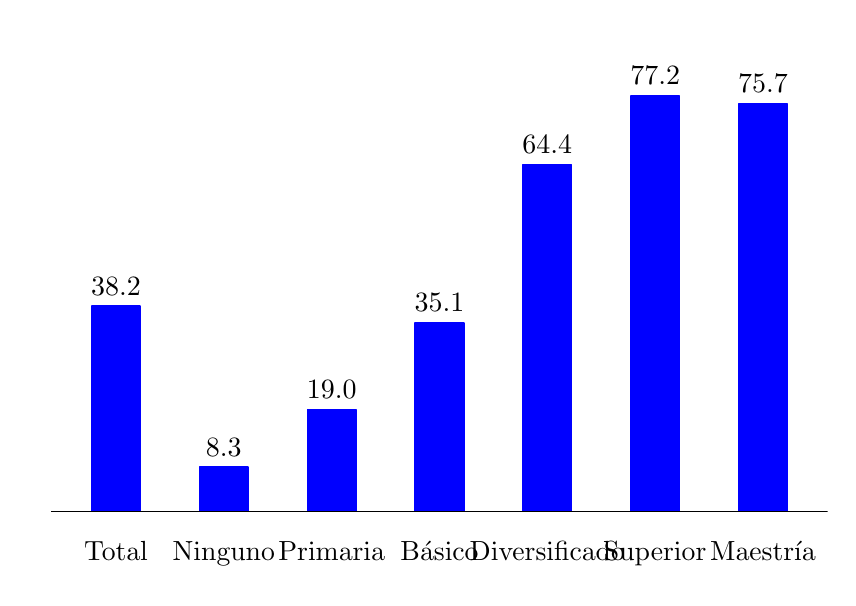
\begin{tikzpicture}[x=1pt,y=1pt]  % Created by tikzDevice version 0.9 on 2015-12-11 10:47:47
% !TEX encoding = UTF-8 Unicode
\definecolor{fillColor}{RGB}{255,255,255}
\path[use as bounding box,fill=fillColor,fill opacity=0.00] (0,0) rectangle (289.08,198.74);
\begin{scope}
\path[clip] (  0.00,  0.00) rectangle (289.08,198.74);

\path[] (  0.00,  0.00) rectangle (289.08,198.74);
\end{scope}
\begin{scope}
\path[clip] (  0.00,  0.00) rectangle (289.08,198.74);

\path[] (  8.54, 16.35) rectangle (289.08,181.67);

\path[] ( 31.91, 16.35) --
	( 31.91,181.67);

\path[] ( 70.88, 16.35) --
	( 70.88,181.67);

\path[] (109.84, 16.35) --
	(109.84,181.67);

\path[] (148.81, 16.35) --
	(148.81,181.67);

\path[] (187.77, 16.35) --
	(187.77,181.67);

\path[] (226.74, 16.35) --
	(226.74,181.67);

\path[] (265.70, 16.35) --
	(265.70,181.67);
\definecolor{drawColor}{RGB}{0,0,255}
\definecolor{fillColor}{RGB}{0,0,255}

\path[draw=drawColor,line width= 0.6pt,line join=round,fill=fillColor] ( 23.15, 23.87) rectangle ( 40.68, 98.18);

\path[draw=drawColor,line width= 0.6pt,line join=round,fill=fillColor] ( 62.11, 23.87) rectangle ( 79.65, 39.95);

\path[draw=drawColor,line width= 0.6pt,line join=round,fill=fillColor] (101.08, 23.87) rectangle (118.61, 60.80);

\path[draw=drawColor,line width= 0.6pt,line join=round,fill=fillColor] (140.04, 23.87) rectangle (157.57, 92.14);

\path[draw=drawColor,line width= 0.6pt,line join=round,fill=fillColor] (179.01, 23.87) rectangle (196.54,149.27);

\path[draw=drawColor,line width= 0.6pt,line join=round,fill=fillColor] (217.97, 23.87) rectangle (235.50,174.16);

\path[draw=drawColor,line width= 0.6pt,line join=round,fill=fillColor] (256.93, 23.87) rectangle (274.47,171.29);
\definecolor{drawColor}{RGB}{0,0,0}

\path[draw=drawColor,line width= 0.1pt,line join=round] (  8.54, 23.87) -- (289.08, 23.87);

\node[text=drawColor,anchor=base,inner sep=0pt, outer sep=0pt, scale=  1.01] at ( 31.91,102.13) {38.2};

\node[text=drawColor,anchor=base,inner sep=0pt, outer sep=0pt, scale=  1.01] at ( 70.88, 43.91) {8.3};

\node[text=drawColor,anchor=base,inner sep=0pt, outer sep=0pt, scale=  1.01] at (109.84, 64.76) {19.0};

\node[text=drawColor,anchor=base,inner sep=0pt, outer sep=0pt, scale=  1.01] at (148.81, 96.10) {35.1};

\node[text=drawColor,anchor=base,inner sep=0pt, outer sep=0pt, scale=  1.01] at (187.77,153.22) {64.4};

\node[text=drawColor,anchor=base,inner sep=0pt, outer sep=0pt, scale=  1.01] at (226.74,178.11) {77.2};

\node[text=drawColor,anchor=base,inner sep=0pt, outer sep=0pt, scale=  1.01] at (265.70,175.25) {75.7};

\path[] (  8.54, 16.35) rectangle (289.08,181.67);
\end{scope}
\begin{scope}
\path[clip] (  0.00,  0.00) rectangle (289.08,198.74);

\path[] (  8.54, 16.35) --
	(  8.54,181.67);
\end{scope}
\begin{scope}
\path[clip] (  0.00,  0.00) rectangle (289.08,198.74);

\path[] (  8.54, 16.35) --
	(289.08, 16.35);
\end{scope}
\begin{scope}
\path[clip] (  0.00,  0.00) rectangle (289.08,198.74);

\path[] ( 31.91, 12.08) --
	( 31.91, 16.35);

\path[] ( 70.88, 12.08) --
	( 70.88, 16.35);

\path[] (109.84, 12.08) --
	(109.84, 16.35);

\path[] (148.81, 12.08) --
	(148.81, 16.35);

\path[] (187.77, 12.08) --
	(187.77, 16.35);

\path[] (226.74, 12.08) --
	(226.74, 16.35);

\path[] (265.70, 12.08) --
	(265.70, 16.35);
\end{scope}
\begin{scope}
\path[clip] (  0.00,  0.00) rectangle (289.08,198.74);
\definecolor{drawColor}{RGB}{0,0,0}

\node[text=drawColor,anchor=base,inner sep=0pt, outer sep=0pt, scale=  1.00] at ( 31.91,  6.04) {Total};

\node[text=drawColor,anchor=base,inner sep=0pt, outer sep=0pt, scale=  1.00] at ( 70.88,  6.04) {Ninguno};

\node[text=drawColor,anchor=base,inner sep=0pt, outer sep=0pt, scale=  1.00] at (109.84,  6.04) {Primaria};

\node[text=drawColor,anchor=base,inner sep=0pt, outer sep=0pt, scale=  1.00] at (148.81,  6.04) {Básico};

\node[text=drawColor,anchor=base,inner sep=0pt, outer sep=0pt, scale=  1.00] at (187.77,  6.04) {Diversificado};

\node[text=drawColor,anchor=base,inner sep=0pt, outer sep=0pt, scale=  1.00] at (226.74,  6.04) {Superior};

\node[text=drawColor,anchor=base,inner sep=0pt, outer sep=0pt, scale=  1.00] at (265.70,  6.04) {Maestría};
\end{scope}
  \end{tikzpicture} }{Instituto Nacional de Estadística, con datos de ENEI II-2014}




\cajita{Asalariados: aguinaldo y escolaridad}{Según el nivel de escolaridad de la población ocupada, el 75.3\% de quienes  tienen educación superior reciben el aguinaldo. Asimismo, de la población sin ningún nivel de escolaridad aprobado, el 7.9\% lo recibe.}{Proporción de la población asalariada que recibe aguinaldo según el nivel de escolaridad}{República de Guatemala, año 2014, en porcentaje}{\ \\[0mm]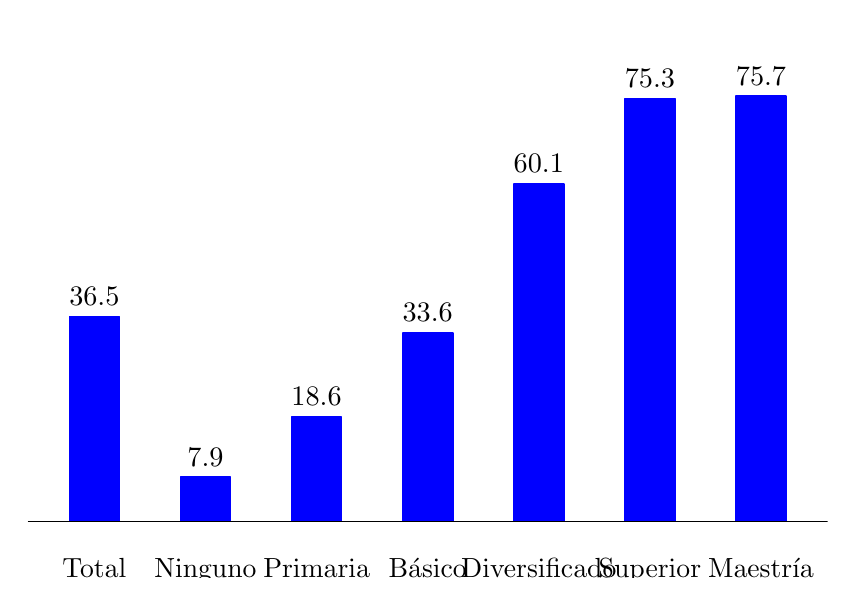
\begin{tikzpicture}[x=1pt,y=1pt]  % Created by tikzDevice version 0.9 on 2016-02-28 17:13:38
% !TEX encoding = UTF-8 Unicode
\definecolor{fillColor}{RGB}{255,255,255}
\path[use as bounding box,fill=fillColor,fill opacity=0.00] (0,0) rectangle (289.08,198.74);
\begin{scope}
\path[clip] (  0.00,  0.00) rectangle (289.08,198.74);

\path[] (  0.00,  0.00) rectangle (289.08,198.74);
\end{scope}
\begin{scope}
\path[clip] (  0.00,  0.00) rectangle (289.08,198.74);

\path[] (  0.00, 12.77) rectangle (289.08,181.67);

\path[] ( 24.09, 12.77) --
	( 24.09,181.67);

\path[] ( 64.24, 12.77) --
	( 64.24,181.67);

\path[] (104.39, 12.77) --
	(104.39,181.67);

\path[] (144.54, 12.77) --
	(144.54,181.67);

\path[] (184.69, 12.77) --
	(184.69,181.67);

\path[] (224.84, 12.77) --
	(224.84,181.67);

\path[] (264.99, 12.77) --
	(264.99,181.67);
\definecolor{drawColor}{RGB}{0,0,255}
\definecolor{fillColor}{RGB}{0,0,255}

\path[draw=drawColor,line width= 0.6pt,line join=round,fill=fillColor] ( 15.06, 20.44) rectangle ( 33.12, 94.41);

\path[draw=drawColor,line width= 0.6pt,line join=round,fill=fillColor] ( 55.21, 20.44) rectangle ( 73.27, 36.38);

\path[draw=drawColor,line width= 0.6pt,line join=round,fill=fillColor] ( 95.36, 20.44) rectangle (113.42, 58.10);

\path[draw=drawColor,line width= 0.6pt,line join=round,fill=fillColor] (135.51, 20.44) rectangle (153.57, 88.48);

\path[draw=drawColor,line width= 0.6pt,line join=round,fill=fillColor] (175.66, 20.44) rectangle (193.72,142.28);

\path[draw=drawColor,line width= 0.6pt,line join=round,fill=fillColor] (215.81, 20.44) rectangle (233.87,173.19);

\path[draw=drawColor,line width= 0.6pt,line join=round,fill=fillColor] (255.96, 20.44) rectangle (274.02,173.99);
\definecolor{drawColor}{RGB}{0,0,0}

\path[draw=drawColor,line width= 0.1pt,line join=round] (  0.00, 20.44) -- (289.08, 20.44);

\node[text=drawColor,anchor=base,inner sep=0pt, outer sep=0pt, scale=  1.02] at ( 24.09, 98.39) {36.5};

\node[text=drawColor,anchor=base,inner sep=0pt, outer sep=0pt, scale=  1.02] at ( 64.24, 40.35) {7.9};

\node[text=drawColor,anchor=base,inner sep=0pt, outer sep=0pt, scale=  1.02] at (104.39, 62.07) {18.6};

\node[text=drawColor,anchor=base,inner sep=0pt, outer sep=0pt, scale=  1.02] at (144.54, 92.45) {33.6};

\node[text=drawColor,anchor=base,inner sep=0pt, outer sep=0pt, scale=  1.02] at (184.69,146.25) {60.1};

\node[text=drawColor,anchor=base,inner sep=0pt, outer sep=0pt, scale=  1.02] at (224.84,177.16) {75.3};

\node[text=drawColor,anchor=base,inner sep=0pt, outer sep=0pt, scale=  1.02] at (264.99,177.96) {75.7};

\path[] (  0.00, 12.77) rectangle (289.08,181.67);
\end{scope}
\begin{scope}
\path[clip] (  0.00,  0.00) rectangle (289.08,198.74);

\path[] (  0.00, 12.77) --
	(289.08, 12.77);
\end{scope}
\begin{scope}
\path[clip] (  0.00,  0.00) rectangle (289.08,198.74);

\path[] ( 24.09, 10.02) --
	( 24.09, 12.77);

\path[] ( 64.24, 10.02) --
	( 64.24, 12.77);

\path[] (104.39, 10.02) --
	(104.39, 12.77);

\path[] (144.54, 10.02) --
	(144.54, 12.77);

\path[] (184.69, 10.02) --
	(184.69, 12.77);

\path[] (224.84, 10.02) --
	(224.84, 12.77);

\path[] (264.99, 10.02) --
	(264.99, 12.77);
\end{scope}
\begin{scope}
\path[clip] (  0.00,  0.00) rectangle (289.08,198.74);
\definecolor{drawColor}{RGB}{0,0,0}

\node[text=drawColor,anchor=base,inner sep=0pt, outer sep=0pt, scale=  1.00] at ( 24.09, -0.00) {Total};

\node[text=drawColor,anchor=base,inner sep=0pt, outer sep=0pt, scale=  1.00] at ( 64.24, -0.00) {Ninguno};

\node[text=drawColor,anchor=base,inner sep=0pt, outer sep=0pt, scale=  1.00] at (104.39, -0.00) {Primaria};

\node[text=drawColor,anchor=base,inner sep=0pt, outer sep=0pt, scale=  1.00] at (144.54, -0.00) {Básico};

\node[text=drawColor,anchor=base,inner sep=0pt, outer sep=0pt, scale=  1.00] at (184.69, -0.00) {Diversificado};

\node[text=drawColor,anchor=base,inner sep=0pt, outer sep=0pt, scale=  1.00] at (224.84, -0.00) {Superior};

\node[text=drawColor,anchor=base,inner sep=0pt, outer sep=0pt, scale=  1.00] at (264.99, -0.00) {Maestría};
\end{scope}
  \end{tikzpicture} }{Instituto Nacional de Estadística, con datos de ENEI II-2014}





\cajita{Escolaridad e ingresos}{Según el nivel de escolaridad de la población ocupada, el nivel de ingresos promedio de quienes  tienen educación superior es de Q4,744.5.  Asimismo, de la población sin ningún nivel de escolaridad aprobado, el promedio de ingresos es de Q1,095.1.}{Promedio de ingresos laborales según el nivel de escolaridad}{República de Guatemala, año 2014, en quetzales corrientes}{\ \\[0mm]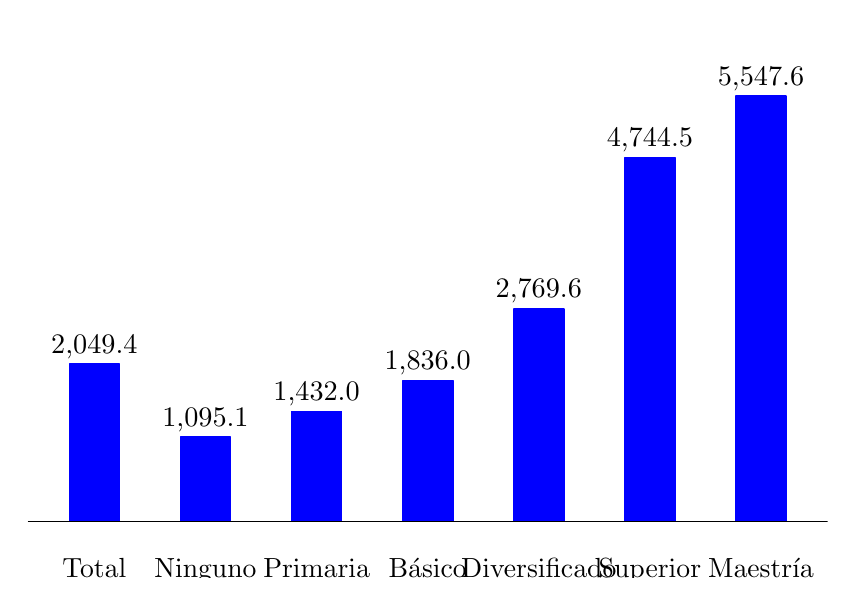
\begin{tikzpicture}[x=1pt,y=1pt]  % Created by tikzDevice version 0.9 on 2016-02-28 17:13:41
% !TEX encoding = UTF-8 Unicode
\definecolor{fillColor}{RGB}{255,255,255}
\path[use as bounding box,fill=fillColor,fill opacity=0.00] (0,0) rectangle (289.08,198.74);
\begin{scope}
\path[clip] (  0.00,  0.00) rectangle (289.08,198.74);

\path[] (  0.00,  0.00) rectangle (289.08,198.74);
\end{scope}
\begin{scope}
\path[clip] (  0.00,  0.00) rectangle (289.08,198.74);

\path[] (  0.00, 12.77) rectangle (289.08,181.67);

\path[] ( 24.09, 12.77) --
	( 24.09,181.67);

\path[] ( 64.24, 12.77) --
	( 64.24,181.67);

\path[] (104.39, 12.77) --
	(104.39,181.67);

\path[] (144.54, 12.77) --
	(144.54,181.67);

\path[] (184.69, 12.77) --
	(184.69,181.67);

\path[] (224.84, 12.77) --
	(224.84,181.67);

\path[] (264.99, 12.77) --
	(264.99,181.67);
\definecolor{drawColor}{RGB}{0,0,255}
\definecolor{fillColor}{RGB}{0,0,255}

\path[draw=drawColor,line width= 0.6pt,line join=round,fill=fillColor] ( 15.06, 20.44) rectangle ( 33.12, 77.17);

\path[draw=drawColor,line width= 0.6pt,line join=round,fill=fillColor] ( 55.21, 20.44) rectangle ( 73.27, 50.75);

\path[draw=drawColor,line width= 0.6pt,line join=round,fill=fillColor] ( 95.36, 20.44) rectangle (113.42, 60.08);

\path[draw=drawColor,line width= 0.6pt,line join=round,fill=fillColor] (135.51, 20.44) rectangle (153.57, 71.26);

\path[draw=drawColor,line width= 0.6pt,line join=round,fill=fillColor] (175.66, 20.44) rectangle (193.72, 97.10);

\path[draw=drawColor,line width= 0.6pt,line join=round,fill=fillColor] (215.81, 20.44) rectangle (233.87,151.77);

\path[draw=drawColor,line width= 0.6pt,line join=round,fill=fillColor] (255.96, 20.44) rectangle (274.02,173.99);
\definecolor{drawColor}{RGB}{0,0,0}

\path[draw=drawColor,line width= 0.1pt,line join=round] (  0.00, 20.44) -- (289.08, 20.44);

\node[text=drawColor,anchor=base,inner sep=0pt, outer sep=0pt, scale=  1.02] at ( 24.09, 81.14) {2,049.4};

\node[text=drawColor,anchor=base,inner sep=0pt, outer sep=0pt, scale=  1.02] at ( 64.24, 54.73) {1,095.1};

\node[text=drawColor,anchor=base,inner sep=0pt, outer sep=0pt, scale=  1.02] at (104.39, 64.05) {1,432.0};

\node[text=drawColor,anchor=base,inner sep=0pt, outer sep=0pt, scale=  1.02] at (144.54, 75.23) {1,836.0};

\node[text=drawColor,anchor=base,inner sep=0pt, outer sep=0pt, scale=  1.02] at (184.69,101.07) {2,769.6};

\node[text=drawColor,anchor=base,inner sep=0pt, outer sep=0pt, scale=  1.02] at (224.84,155.74) {4,744.5};

\node[text=drawColor,anchor=base,inner sep=0pt, outer sep=0pt, scale=  1.02] at (264.99,177.96) {5,547.6};

\path[] (  0.00, 12.77) rectangle (289.08,181.67);
\end{scope}
\begin{scope}
\path[clip] (  0.00,  0.00) rectangle (289.08,198.74);

\path[] (  0.00, 12.77) --
	(289.08, 12.77);
\end{scope}
\begin{scope}
\path[clip] (  0.00,  0.00) rectangle (289.08,198.74);

\path[] ( 24.09, 10.02) --
	( 24.09, 12.77);

\path[] ( 64.24, 10.02) --
	( 64.24, 12.77);

\path[] (104.39, 10.02) --
	(104.39, 12.77);

\path[] (144.54, 10.02) --
	(144.54, 12.77);

\path[] (184.69, 10.02) --
	(184.69, 12.77);

\path[] (224.84, 10.02) --
	(224.84, 12.77);

\path[] (264.99, 10.02) --
	(264.99, 12.77);
\end{scope}
\begin{scope}
\path[clip] (  0.00,  0.00) rectangle (289.08,198.74);
\definecolor{drawColor}{RGB}{0,0,0}

\node[text=drawColor,anchor=base,inner sep=0pt, outer sep=0pt, scale=  1.00] at ( 24.09, -0.00) {Total};

\node[text=drawColor,anchor=base,inner sep=0pt, outer sep=0pt, scale=  1.00] at ( 64.24, -0.00) {Ninguno};

\node[text=drawColor,anchor=base,inner sep=0pt, outer sep=0pt, scale=  1.00] at (104.39, -0.00) {Primaria};

\node[text=drawColor,anchor=base,inner sep=0pt, outer sep=0pt, scale=  1.00] at (144.54, -0.00) {Básico};

\node[text=drawColor,anchor=base,inner sep=0pt, outer sep=0pt, scale=  1.00] at (184.69, -0.00) {Diversificado};

\node[text=drawColor,anchor=base,inner sep=0pt, outer sep=0pt, scale=  1.00] at (224.84, -0.00) {Superior};

\node[text=drawColor,anchor=base,inner sep=0pt, outer sep=0pt, scale=  1.00] at (264.99, -0.00) {Maestría};
\end{scope}
  \end{tikzpicture} }{Instituto Nacional de Estadística, con datos de ENEI II-2014}



\cajita{Escolaridad e ingresos, según sexo}{Según el nivel de escolaridad de la población ocupada por sexo, el nivel de ingresos promedio de los hombres con  educación superior es de Q5,652.3, siendo el mayor de la serie.
	
	  Asimismo,  el menor promedio de ingresos se encuentra en las mujeres que no cuentan con ningún nivel de educación aprobado, siendo este de Q758.4.}{Promedio de ingresos laborales según el nivel de escolaridad y sexo}{República de Guatemala, año 2014, en quetzales corrientes}{\ \\[0mm]\begin{tikzpicture}[x=1pt,y=1pt]  % Created by tikzDevice version 0.9 on 2015-12-11 10:47:48
% !TEX encoding = UTF-8 Unicode
\definecolor{fillColor}{RGB}{255,255,255}
\path[use as bounding box,fill=fillColor,fill opacity=0.00] (0,0) rectangle (289.08,198.74);
\begin{scope}
\path[clip] (  0.00,  0.00) rectangle (289.08,198.74);

\path[] (  0.00,  0.00) rectangle (289.08,198.74);
\end{scope}
\begin{scope}
\path[clip] (  0.00,  0.00) rectangle (289.08,198.74);

\path[] (  7.11, 20.62) rectangle (289.08,172.85);

\path[] ( 34.40, 20.62) --
	( 34.40,172.85);

\path[] ( 79.88, 20.62) --
	( 79.88,172.85);

\path[] (125.36, 20.62) --
	(125.36,172.85);

\path[] (170.84, 20.62) --
	(170.84,172.85);

\path[] (216.31, 20.62) --
	(216.31,172.85);

\path[] (261.79, 20.62) --
	(261.79,172.85);
\definecolor{drawColor}{RGB}{0,0,255}
\definecolor{fillColor}{RGB}{0,0,255}

\path[draw=drawColor,line width= 0.6pt,line join=round,fill=fillColor] ( 16.78, 20.62) rectangle ( 31.56, 76.84);
\definecolor{drawColor}{RGB}{157,187,255}
\definecolor{fillColor}{RGB}{157,187,255}

\path[draw=drawColor,line width= 0.6pt,line join=round,fill=fillColor] ( 37.24, 20.62) rectangle ( 52.02, 73.63);
\definecolor{drawColor}{RGB}{0,0,255}
\definecolor{fillColor}{RGB}{0,0,255}

\path[draw=drawColor,line width= 0.6pt,line join=round,fill=fillColor] ( 62.26, 20.62) rectangle ( 77.04, 52.84);
\definecolor{drawColor}{RGB}{157,187,255}
\definecolor{fillColor}{RGB}{157,187,255}

\path[draw=drawColor,line width= 0.6pt,line join=round,fill=fillColor] ( 82.72, 20.62) rectangle ( 97.50, 41.04);
\definecolor{drawColor}{RGB}{0,0,255}
\definecolor{fillColor}{RGB}{0,0,255}

\path[draw=drawColor,line width= 0.6pt,line join=round,fill=fillColor] (107.73, 20.62) rectangle (122.51, 61.52);
\definecolor{drawColor}{RGB}{157,187,255}
\definecolor{fillColor}{RGB}{157,187,255}

\path[draw=drawColor,line width= 0.6pt,line join=round,fill=fillColor] (128.20, 20.62) rectangle (142.98, 51.44);
\definecolor{drawColor}{RGB}{0,0,255}
\definecolor{fillColor}{RGB}{0,0,255}

\path[draw=drawColor,line width= 0.6pt,line join=round,fill=fillColor] (153.21, 20.62) rectangle (167.99, 71.96);
\definecolor{drawColor}{RGB}{157,187,255}
\definecolor{fillColor}{RGB}{157,187,255}

\path[draw=drawColor,line width= 0.6pt,line join=round,fill=fillColor] (173.68, 20.62) rectangle (188.46, 64.71);
\definecolor{drawColor}{RGB}{0,0,255}
\definecolor{fillColor}{RGB}{0,0,255}

\path[draw=drawColor,line width= 0.6pt,line join=round,fill=fillColor] (198.69, 20.62) rectangle (213.47, 96.43);
\definecolor{drawColor}{RGB}{157,187,255}
\definecolor{fillColor}{RGB}{157,187,255}

\path[draw=drawColor,line width= 0.6pt,line join=round,fill=fillColor] (219.16, 20.62) rectangle (233.94, 93.50);
\definecolor{drawColor}{RGB}{0,0,255}
\definecolor{fillColor}{RGB}{0,0,255}

\path[draw=drawColor,line width= 0.6pt,line join=round,fill=fillColor] (244.17, 20.62) rectangle (258.95,172.85);
\definecolor{drawColor}{RGB}{157,187,255}
\definecolor{fillColor}{RGB}{157,187,255}

\path[draw=drawColor,line width= 0.6pt,line join=round,fill=fillColor] (264.64, 20.62) rectangle (279.42,120.13);
\definecolor{drawColor}{RGB}{0,0,0}

\path[draw=drawColor,line width= 0.6pt,line join=round] (  7.11, 20.62) -- (289.08, 20.62);

\node[text=drawColor,anchor=base,inner sep=0pt, outer sep=0pt, scale=  0.82] at ( 24.17, 80.06) {2,087.3};

\node[text=drawColor,anchor=base,inner sep=0pt, outer sep=0pt, scale=  0.82] at ( 44.63, 76.86) {1,968.4};

\node[text=drawColor,anchor=base,inner sep=0pt, outer sep=0pt, scale=  0.82] at ( 69.65, 56.06) {1,196.2};

\node[text=drawColor,anchor=base,inner sep=0pt, outer sep=0pt, scale=  0.82] at ( 90.11, 44.27) {758.4};

\node[text=drawColor,anchor=base,inner sep=0pt, outer sep=0pt, scale=  0.82] at (115.12, 64.74) {1,518.6};

\node[text=drawColor,anchor=base,inner sep=0pt, outer sep=0pt, scale=  0.82] at (135.59, 54.67) {1,144.5};

\node[text=drawColor,anchor=base,inner sep=0pt, outer sep=0pt, scale=  0.82] at (160.60, 75.18) {1,906.2};

\node[text=drawColor,anchor=base,inner sep=0pt, outer sep=0pt, scale=  0.82] at (181.07, 67.94) {1,637.2};

\node[text=drawColor,anchor=base,inner sep=0pt, outer sep=0pt, scale=  0.82] at (206.08, 99.65) {2,814.7};

\node[text=drawColor,anchor=base,inner sep=0pt, outer sep=0pt, scale=  0.82] at (226.55, 96.72) {2,705.9};

\node[text=drawColor,anchor=base,inner sep=0pt, outer sep=0pt, scale=  0.82] at (251.56,176.07) {5,652.3};

\node[text=drawColor,anchor=base,inner sep=0pt, outer sep=0pt, scale=  0.82] at (272.03,123.35) {3,694.8};

\path[] (  7.11, 20.62) rectangle (289.08,172.85);
\end{scope}
\begin{scope}
\path[clip] (  0.00,  0.00) rectangle (289.08,198.74);

\path[] (  7.11, 20.62) --
	(  7.11,172.85);
\end{scope}
\begin{scope}
\path[clip] (  0.00,  0.00) rectangle (289.08,198.74);

\path[] (  7.11, 20.62) --
	(289.08, 20.62);
\end{scope}
\begin{scope}
\path[clip] (  0.00,  0.00) rectangle (289.08,198.74);

\path[] ( 34.40, 16.35) --
	( 34.40, 20.62);

\path[] ( 79.88, 16.35) --
	( 79.88, 20.62);

\path[] (125.36, 16.35) --
	(125.36, 20.62);

\path[] (170.84, 16.35) --
	(170.84, 20.62);

\path[] (216.31, 16.35) --
	(216.31, 20.62);

\path[] (261.79, 16.35) --
	(261.79, 20.62);
\end{scope}
\begin{scope}
\path[clip] (  0.00,  0.00) rectangle (289.08,198.74);
\definecolor{drawColor}{RGB}{0,0,0}

\node[text=drawColor,anchor=base,inner sep=0pt, outer sep=0pt, scale=  1.00] at ( 34.40,  5.69) {Total};

\node[text=drawColor,anchor=base,inner sep=0pt, outer sep=0pt, scale=  1.00] at ( 79.88,  5.69) {Ninguno};

\node[text=drawColor,anchor=base,inner sep=0pt, outer sep=0pt, scale=  1.00] at (125.36,  5.69) {Primaria};

\node[text=drawColor,anchor=base,inner sep=0pt, outer sep=0pt, scale=  1.00] at (170.84,  5.69) {Básico};

\node[text=drawColor,anchor=base,inner sep=0pt, outer sep=0pt, scale=  1.00] at (216.31,  5.69) {Diversificado};

\node[text=drawColor,anchor=base,inner sep=0pt, outer sep=0pt, scale=  1.00] at (261.79,  5.69) {Superior};
\end{scope}
\begin{scope}
\path[clip] (  0.00,  0.00) rectangle (289.08,198.74);
\coordinate (apoyo) at (55.98,189.21);
\coordinate (longitudFicticia) at (7.11,9.53);
\coordinate (longitud) at (7.11,7.11);
\coordinate (desX) at (142.21,0);
\coordinate (desY) at (0,1.21);
\definecolor[named]{ct1}{HTML}{
0000FF
}
\definecolor[named]{ct2}{HTML}{
9DBBFF
}
\definecolor[named]{ctb1}{HTML}{
0000FF
}
\definecolor[named]{ctb2}{HTML}{
9DBBFF
}
\path [fill=none] (apoyo) rectangle ($(apoyo)+(longitudFicticia)$)
node [xshift=0.3cm,inner sep=0pt, outer sep=0pt,midway,right,scale = 0.9]{Hombre};
\draw [color = ctb1,fill=ct1] ( $(apoyo)  + (desY) $) rectangle ($(apoyo)+ (desY) +(longitud)$);
\path [fill=none] ($(apoyo)+(desX)$) rectangle ($(apoyo)+(desX)+(longitudFicticia)$)
node [xshift=0.3cm,inner sep=0pt, outer sep=0pt,midway,right,scale = 0.9]{Mujer};
\draw [color = ctb2 ,fill=ct2] ( $(apoyo)  + (desY) + (desX) $) rectangle ($(apoyo)+ (desY)+ (desX) +(longitud)$);
\end{scope}
  \end{tikzpicture} }{Instituto Nacional de Estadística, con datos de ENEI II-2014}

%
%
%\cajita{Desempleo}{La tasa de desempleo abierto se ha mantenido entre el 2.9 y 4.1\%.
%	
%	 En desempleo abierto se consideran a las personas que no laboran pero que están buscando trabajo, estas forman parte de la población económicamente activa.}{Tasa de desempleo abierto}{República de Guatemala, serie histórica, en porcentaje}{\ \\[0mm]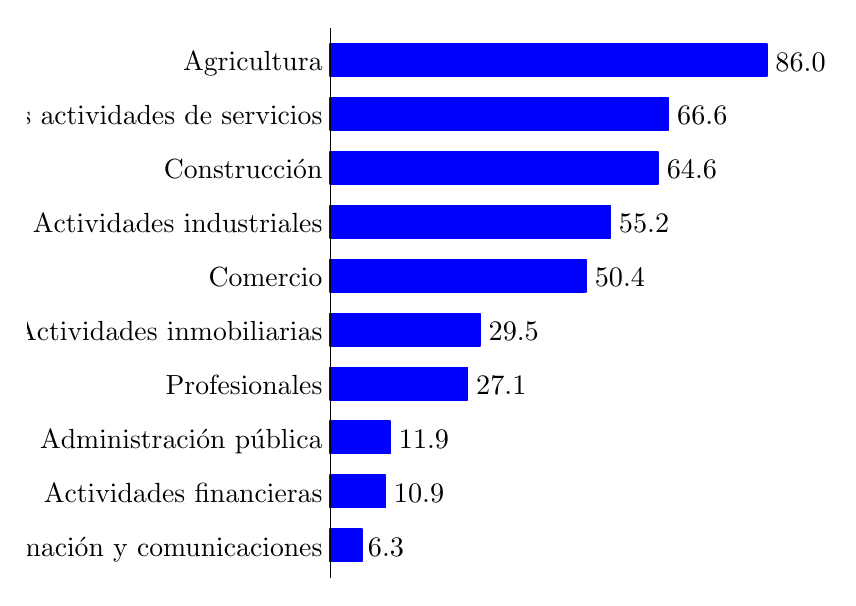
\begin{tikzpicture}[x=1pt,y=1pt]  % Created by tikzDevice version 0.9 on 2016-02-28 20:01:55
% !TEX encoding = UTF-8 Unicode
\definecolor{fillColor}{RGB}{255,255,255}
\path[use as bounding box,fill=fillColor,fill opacity=0.00] (0,0) rectangle (289.08,198.74);
\begin{scope}
\path[clip] (  0.00,  0.00) rectangle (289.08,198.74);

\path[] (  0.00,  0.00) rectangle (289.08,198.74);
\end{scope}
\begin{scope}
\path[clip] (  0.00,  0.00) rectangle (289.08,198.74);

\path[] (109.26,  0.00) rectangle (267.09,198.74);

\path[] (109.26, 11.69) --
	(267.09, 11.69);

\path[] (109.26, 31.18) --
	(267.09, 31.18);

\path[] (109.26, 50.66) --
	(267.09, 50.66);

\path[] (109.26, 70.14) --
	(267.09, 70.14);

\path[] (109.26, 89.63) --
	(267.09, 89.63);

\path[] (109.26,109.11) --
	(267.09,109.11);

\path[] (109.26,128.60) --
	(267.09,128.60);

\path[] (109.26,148.08) --
	(267.09,148.08);

\path[] (109.26,167.57) --
	(267.09,167.57);

\path[] (109.26,187.05) --
	(267.09,187.05);
\definecolor{drawColor}{RGB}{0,0,255}
\definecolor{fillColor}{RGB}{0,0,255}

\path[draw=drawColor,line width= 0.6pt,line join=round,fill=fillColor] (109.26,  5.85) rectangle (120.73, 17.54);

\path[draw=drawColor,line width= 0.6pt,line join=round,fill=fillColor] (109.26, 25.33) rectangle (129.25, 37.02);

\path[draw=drawColor,line width= 0.6pt,line join=round,fill=fillColor] (109.26, 44.81) rectangle (131.02, 56.51);

\path[draw=drawColor,line width= 0.6pt,line join=round,fill=fillColor] (109.26, 64.30) rectangle (158.94, 75.99);

\path[draw=drawColor,line width= 0.6pt,line join=round,fill=fillColor] (109.26, 83.78) rectangle (163.45, 95.47);

\path[draw=drawColor,line width= 0.6pt,line join=round,fill=fillColor] (109.26,103.27) rectangle (201.80,114.96);

\path[draw=drawColor,line width= 0.6pt,line join=round,fill=fillColor] (109.26,122.75) rectangle (210.55,134.44);

\path[draw=drawColor,line width= 0.6pt,line join=round,fill=fillColor] (109.26,142.24) rectangle (227.82,153.93);

\path[draw=drawColor,line width= 0.6pt,line join=round,fill=fillColor] (109.26,161.72) rectangle (231.57,173.41);

\path[draw=drawColor,line width= 0.6pt,line join=round,fill=fillColor] (109.26,181.21) rectangle (267.09,192.90);
\definecolor{drawColor}{RGB}{0,0,0}

\path[draw=drawColor,line width= 0.1pt,line join=round] (109.26,  0.00) -- (109.26,198.74);

\node[text=drawColor,anchor=base west,inner sep=0pt, outer sep=0pt, scale=  1.02] at (122.97,  7.72) {6.3};

\node[text=drawColor,anchor=base west,inner sep=0pt, outer sep=0pt, scale=  1.02] at (132.37, 27.20) {10.9};

\node[text=drawColor,anchor=base west,inner sep=0pt, outer sep=0pt, scale=  1.02] at (134.15, 46.69) {11.9};

\node[text=drawColor,anchor=base west,inner sep=0pt, outer sep=0pt, scale=  1.02] at (162.07, 66.17) {27.1};

\node[text=drawColor,anchor=base west,inner sep=0pt, outer sep=0pt, scale=  1.02] at (166.58, 85.66) {29.5};

\node[text=drawColor,anchor=base west,inner sep=0pt, outer sep=0pt, scale=  1.02] at (204.93,105.14) {50.4};

\node[text=drawColor,anchor=base west,inner sep=0pt, outer sep=0pt, scale=  1.02] at (213.67,124.63) {55.2};

\node[text=drawColor,anchor=base west,inner sep=0pt, outer sep=0pt, scale=  1.02] at (230.95,144.11) {64.6};

\node[text=drawColor,anchor=base west,inner sep=0pt, outer sep=0pt, scale=  1.02] at (234.70,163.60) {66.6};

\node[text=drawColor,anchor=base west,inner sep=0pt, outer sep=0pt, scale=  1.02] at (270.21,183.08) {86.0};

\path[] (109.26,  0.00) rectangle (267.09,198.74);
\end{scope}
\begin{scope}
\path[clip] (  0.00,  0.00) rectangle (289.08,198.74);

\path[] (109.26,  0.00) --
	(109.26,198.74);
\end{scope}
\begin{scope}
\path[clip] (  0.00,  0.00) rectangle (289.08,198.74);
\definecolor{drawColor}{RGB}{0,0,0}

\node[text=drawColor,anchor=base east,inner sep=0pt, outer sep=0pt, scale=  1.00] at (106.51,  7.78) {Información y comunicaciones};

\node[text=drawColor,anchor=base east,inner sep=0pt, outer sep=0pt, scale=  1.00] at (106.51, 27.27) {Actividades financieras };

\node[text=drawColor,anchor=base east,inner sep=0pt, outer sep=0pt, scale=  1.00] at (106.51, 46.75) {Administración pública };

\node[text=drawColor,anchor=base east,inner sep=0pt, outer sep=0pt, scale=  1.00] at (106.51, 66.24) {Profesionales};

\node[text=drawColor,anchor=base east,inner sep=0pt, outer sep=0pt, scale=  1.00] at (106.51, 85.72) {Actividades inmobiliarias};

\node[text=drawColor,anchor=base east,inner sep=0pt, outer sep=0pt, scale=  1.00] at (106.51,105.21) {Comercio };

\node[text=drawColor,anchor=base east,inner sep=0pt, outer sep=0pt, scale=  1.00] at (106.51,124.69) {Actividades  industriales};

\node[text=drawColor,anchor=base east,inner sep=0pt, outer sep=0pt, scale=  1.00] at (106.51,144.17) {Construcción};

\node[text=drawColor,anchor=base east,inner sep=0pt, outer sep=0pt, scale=  1.00] at (106.51,163.66) {Otras actividades de servicios};

\node[text=drawColor,anchor=base east,inner sep=0pt, outer sep=0pt, scale=  1.00] at (106.51,183.14) {Agricultura};
\end{scope}
\begin{scope}
\path[clip] (  0.00,  0.00) rectangle (289.08,198.74);

\path[] (106.51, 11.69) --
	(109.26, 11.69);

\path[] (106.51, 31.18) --
	(109.26, 31.18);

\path[] (106.51, 50.66) --
	(109.26, 50.66);

\path[] (106.51, 70.14) --
	(109.26, 70.14);

\path[] (106.51, 89.63) --
	(109.26, 89.63);

\path[] (106.51,109.11) --
	(109.26,109.11);

\path[] (106.51,128.60) --
	(109.26,128.60);

\path[] (106.51,148.08) --
	(109.26,148.08);

\path[] (106.51,167.57) --
	(109.26,167.57);

\path[] (106.51,187.05) --
	(109.26,187.05);
\end{scope}
  \end{tikzpicture} }{Instituto Nacional de Estadística, con datos de ENEI II-2014}


%
%\cajita{Desempleo según sexo}{}{Tasa de desempleo abierto según sexo}{República de Guatemala, año 2014, en porcentaje}{\ \\[0mm]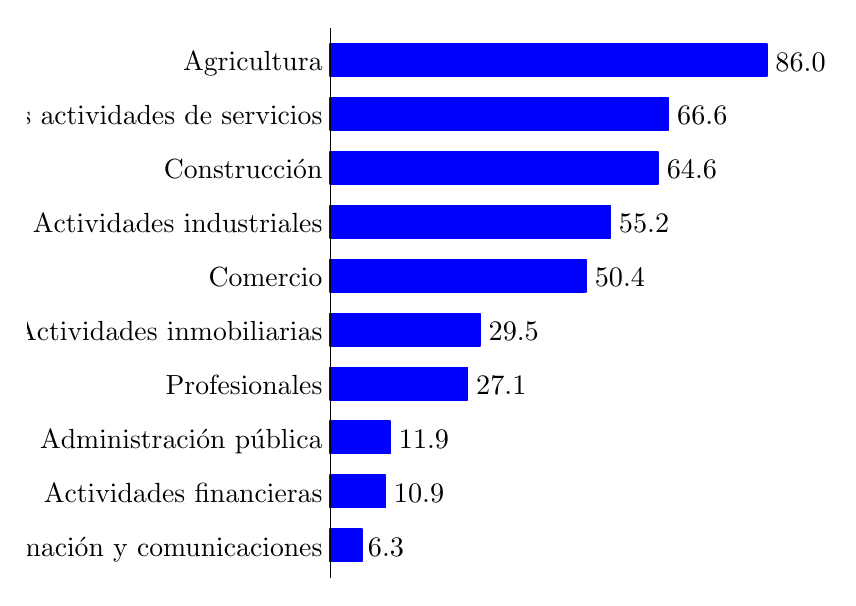
\begin{tikzpicture}[x=1pt,y=1pt]  % Created by tikzDevice version 0.9 on 2016-02-28 20:01:55
% !TEX encoding = UTF-8 Unicode
\definecolor{fillColor}{RGB}{255,255,255}
\path[use as bounding box,fill=fillColor,fill opacity=0.00] (0,0) rectangle (289.08,198.74);
\begin{scope}
\path[clip] (  0.00,  0.00) rectangle (289.08,198.74);

\path[] (  0.00,  0.00) rectangle (289.08,198.74);
\end{scope}
\begin{scope}
\path[clip] (  0.00,  0.00) rectangle (289.08,198.74);

\path[] (109.26,  0.00) rectangle (267.09,198.74);

\path[] (109.26, 11.69) --
	(267.09, 11.69);

\path[] (109.26, 31.18) --
	(267.09, 31.18);

\path[] (109.26, 50.66) --
	(267.09, 50.66);

\path[] (109.26, 70.14) --
	(267.09, 70.14);

\path[] (109.26, 89.63) --
	(267.09, 89.63);

\path[] (109.26,109.11) --
	(267.09,109.11);

\path[] (109.26,128.60) --
	(267.09,128.60);

\path[] (109.26,148.08) --
	(267.09,148.08);

\path[] (109.26,167.57) --
	(267.09,167.57);

\path[] (109.26,187.05) --
	(267.09,187.05);
\definecolor{drawColor}{RGB}{0,0,255}
\definecolor{fillColor}{RGB}{0,0,255}

\path[draw=drawColor,line width= 0.6pt,line join=round,fill=fillColor] (109.26,  5.85) rectangle (120.73, 17.54);

\path[draw=drawColor,line width= 0.6pt,line join=round,fill=fillColor] (109.26, 25.33) rectangle (129.25, 37.02);

\path[draw=drawColor,line width= 0.6pt,line join=round,fill=fillColor] (109.26, 44.81) rectangle (131.02, 56.51);

\path[draw=drawColor,line width= 0.6pt,line join=round,fill=fillColor] (109.26, 64.30) rectangle (158.94, 75.99);

\path[draw=drawColor,line width= 0.6pt,line join=round,fill=fillColor] (109.26, 83.78) rectangle (163.45, 95.47);

\path[draw=drawColor,line width= 0.6pt,line join=round,fill=fillColor] (109.26,103.27) rectangle (201.80,114.96);

\path[draw=drawColor,line width= 0.6pt,line join=round,fill=fillColor] (109.26,122.75) rectangle (210.55,134.44);

\path[draw=drawColor,line width= 0.6pt,line join=round,fill=fillColor] (109.26,142.24) rectangle (227.82,153.93);

\path[draw=drawColor,line width= 0.6pt,line join=round,fill=fillColor] (109.26,161.72) rectangle (231.57,173.41);

\path[draw=drawColor,line width= 0.6pt,line join=round,fill=fillColor] (109.26,181.21) rectangle (267.09,192.90);
\definecolor{drawColor}{RGB}{0,0,0}

\path[draw=drawColor,line width= 0.1pt,line join=round] (109.26,  0.00) -- (109.26,198.74);

\node[text=drawColor,anchor=base west,inner sep=0pt, outer sep=0pt, scale=  1.02] at (122.97,  7.72) {6.3};

\node[text=drawColor,anchor=base west,inner sep=0pt, outer sep=0pt, scale=  1.02] at (132.37, 27.20) {10.9};

\node[text=drawColor,anchor=base west,inner sep=0pt, outer sep=0pt, scale=  1.02] at (134.15, 46.69) {11.9};

\node[text=drawColor,anchor=base west,inner sep=0pt, outer sep=0pt, scale=  1.02] at (162.07, 66.17) {27.1};

\node[text=drawColor,anchor=base west,inner sep=0pt, outer sep=0pt, scale=  1.02] at (166.58, 85.66) {29.5};

\node[text=drawColor,anchor=base west,inner sep=0pt, outer sep=0pt, scale=  1.02] at (204.93,105.14) {50.4};

\node[text=drawColor,anchor=base west,inner sep=0pt, outer sep=0pt, scale=  1.02] at (213.67,124.63) {55.2};

\node[text=drawColor,anchor=base west,inner sep=0pt, outer sep=0pt, scale=  1.02] at (230.95,144.11) {64.6};

\node[text=drawColor,anchor=base west,inner sep=0pt, outer sep=0pt, scale=  1.02] at (234.70,163.60) {66.6};

\node[text=drawColor,anchor=base west,inner sep=0pt, outer sep=0pt, scale=  1.02] at (270.21,183.08) {86.0};

\path[] (109.26,  0.00) rectangle (267.09,198.74);
\end{scope}
\begin{scope}
\path[clip] (  0.00,  0.00) rectangle (289.08,198.74);

\path[] (109.26,  0.00) --
	(109.26,198.74);
\end{scope}
\begin{scope}
\path[clip] (  0.00,  0.00) rectangle (289.08,198.74);
\definecolor{drawColor}{RGB}{0,0,0}

\node[text=drawColor,anchor=base east,inner sep=0pt, outer sep=0pt, scale=  1.00] at (106.51,  7.78) {Información y comunicaciones};

\node[text=drawColor,anchor=base east,inner sep=0pt, outer sep=0pt, scale=  1.00] at (106.51, 27.27) {Actividades financieras };

\node[text=drawColor,anchor=base east,inner sep=0pt, outer sep=0pt, scale=  1.00] at (106.51, 46.75) {Administración pública };

\node[text=drawColor,anchor=base east,inner sep=0pt, outer sep=0pt, scale=  1.00] at (106.51, 66.24) {Profesionales};

\node[text=drawColor,anchor=base east,inner sep=0pt, outer sep=0pt, scale=  1.00] at (106.51, 85.72) {Actividades inmobiliarias};

\node[text=drawColor,anchor=base east,inner sep=0pt, outer sep=0pt, scale=  1.00] at (106.51,105.21) {Comercio };

\node[text=drawColor,anchor=base east,inner sep=0pt, outer sep=0pt, scale=  1.00] at (106.51,124.69) {Actividades  industriales};

\node[text=drawColor,anchor=base east,inner sep=0pt, outer sep=0pt, scale=  1.00] at (106.51,144.17) {Construcción};

\node[text=drawColor,anchor=base east,inner sep=0pt, outer sep=0pt, scale=  1.00] at (106.51,163.66) {Otras actividades de servicios};

\node[text=drawColor,anchor=base east,inner sep=0pt, outer sep=0pt, scale=  1.00] at (106.51,183.14) {Agricultura};
\end{scope}
\begin{scope}
\path[clip] (  0.00,  0.00) rectangle (289.08,198.74);

\path[] (106.51, 11.69) --
	(109.26, 11.69);

\path[] (106.51, 31.18) --
	(109.26, 31.18);

\path[] (106.51, 50.66) --
	(109.26, 50.66);

\path[] (106.51, 70.14) --
	(109.26, 70.14);

\path[] (106.51, 89.63) --
	(109.26, 89.63);

\path[] (106.51,109.11) --
	(109.26,109.11);

\path[] (106.51,128.60) --
	(109.26,128.60);

\path[] (106.51,148.08) --
	(109.26,148.08);

\path[] (106.51,167.57) --
	(109.26,167.57);

\path[] (106.51,187.05) --
	(109.26,187.05);
\end{scope}
  \end{tikzpicture} }{Instituto Nacional de Estadística, con datos de ENEI II-2014}
%
%
%\cajita{Desocupados analfabetos según dominio}{}{Proporción de la población desocupada que es analfabeta, por dominio de estudio}{República de Guatemala, año 2014, en porcentaje}{\ \\[0mm]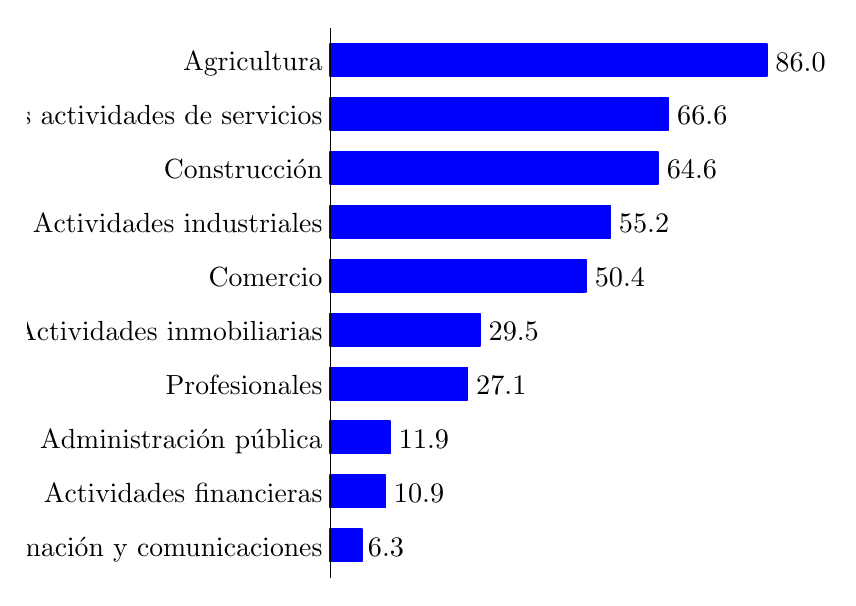
\begin{tikzpicture}[x=1pt,y=1pt]  % Created by tikzDevice version 0.9 on 2016-02-28 20:01:55
% !TEX encoding = UTF-8 Unicode
\definecolor{fillColor}{RGB}{255,255,255}
\path[use as bounding box,fill=fillColor,fill opacity=0.00] (0,0) rectangle (289.08,198.74);
\begin{scope}
\path[clip] (  0.00,  0.00) rectangle (289.08,198.74);

\path[] (  0.00,  0.00) rectangle (289.08,198.74);
\end{scope}
\begin{scope}
\path[clip] (  0.00,  0.00) rectangle (289.08,198.74);

\path[] (109.26,  0.00) rectangle (267.09,198.74);

\path[] (109.26, 11.69) --
	(267.09, 11.69);

\path[] (109.26, 31.18) --
	(267.09, 31.18);

\path[] (109.26, 50.66) --
	(267.09, 50.66);

\path[] (109.26, 70.14) --
	(267.09, 70.14);

\path[] (109.26, 89.63) --
	(267.09, 89.63);

\path[] (109.26,109.11) --
	(267.09,109.11);

\path[] (109.26,128.60) --
	(267.09,128.60);

\path[] (109.26,148.08) --
	(267.09,148.08);

\path[] (109.26,167.57) --
	(267.09,167.57);

\path[] (109.26,187.05) --
	(267.09,187.05);
\definecolor{drawColor}{RGB}{0,0,255}
\definecolor{fillColor}{RGB}{0,0,255}

\path[draw=drawColor,line width= 0.6pt,line join=round,fill=fillColor] (109.26,  5.85) rectangle (120.73, 17.54);

\path[draw=drawColor,line width= 0.6pt,line join=round,fill=fillColor] (109.26, 25.33) rectangle (129.25, 37.02);

\path[draw=drawColor,line width= 0.6pt,line join=round,fill=fillColor] (109.26, 44.81) rectangle (131.02, 56.51);

\path[draw=drawColor,line width= 0.6pt,line join=round,fill=fillColor] (109.26, 64.30) rectangle (158.94, 75.99);

\path[draw=drawColor,line width= 0.6pt,line join=round,fill=fillColor] (109.26, 83.78) rectangle (163.45, 95.47);

\path[draw=drawColor,line width= 0.6pt,line join=round,fill=fillColor] (109.26,103.27) rectangle (201.80,114.96);

\path[draw=drawColor,line width= 0.6pt,line join=round,fill=fillColor] (109.26,122.75) rectangle (210.55,134.44);

\path[draw=drawColor,line width= 0.6pt,line join=round,fill=fillColor] (109.26,142.24) rectangle (227.82,153.93);

\path[draw=drawColor,line width= 0.6pt,line join=round,fill=fillColor] (109.26,161.72) rectangle (231.57,173.41);

\path[draw=drawColor,line width= 0.6pt,line join=round,fill=fillColor] (109.26,181.21) rectangle (267.09,192.90);
\definecolor{drawColor}{RGB}{0,0,0}

\path[draw=drawColor,line width= 0.1pt,line join=round] (109.26,  0.00) -- (109.26,198.74);

\node[text=drawColor,anchor=base west,inner sep=0pt, outer sep=0pt, scale=  1.02] at (122.97,  7.72) {6.3};

\node[text=drawColor,anchor=base west,inner sep=0pt, outer sep=0pt, scale=  1.02] at (132.37, 27.20) {10.9};

\node[text=drawColor,anchor=base west,inner sep=0pt, outer sep=0pt, scale=  1.02] at (134.15, 46.69) {11.9};

\node[text=drawColor,anchor=base west,inner sep=0pt, outer sep=0pt, scale=  1.02] at (162.07, 66.17) {27.1};

\node[text=drawColor,anchor=base west,inner sep=0pt, outer sep=0pt, scale=  1.02] at (166.58, 85.66) {29.5};

\node[text=drawColor,anchor=base west,inner sep=0pt, outer sep=0pt, scale=  1.02] at (204.93,105.14) {50.4};

\node[text=drawColor,anchor=base west,inner sep=0pt, outer sep=0pt, scale=  1.02] at (213.67,124.63) {55.2};

\node[text=drawColor,anchor=base west,inner sep=0pt, outer sep=0pt, scale=  1.02] at (230.95,144.11) {64.6};

\node[text=drawColor,anchor=base west,inner sep=0pt, outer sep=0pt, scale=  1.02] at (234.70,163.60) {66.6};

\node[text=drawColor,anchor=base west,inner sep=0pt, outer sep=0pt, scale=  1.02] at (270.21,183.08) {86.0};

\path[] (109.26,  0.00) rectangle (267.09,198.74);
\end{scope}
\begin{scope}
\path[clip] (  0.00,  0.00) rectangle (289.08,198.74);

\path[] (109.26,  0.00) --
	(109.26,198.74);
\end{scope}
\begin{scope}
\path[clip] (  0.00,  0.00) rectangle (289.08,198.74);
\definecolor{drawColor}{RGB}{0,0,0}

\node[text=drawColor,anchor=base east,inner sep=0pt, outer sep=0pt, scale=  1.00] at (106.51,  7.78) {Información y comunicaciones};

\node[text=drawColor,anchor=base east,inner sep=0pt, outer sep=0pt, scale=  1.00] at (106.51, 27.27) {Actividades financieras };

\node[text=drawColor,anchor=base east,inner sep=0pt, outer sep=0pt, scale=  1.00] at (106.51, 46.75) {Administración pública };

\node[text=drawColor,anchor=base east,inner sep=0pt, outer sep=0pt, scale=  1.00] at (106.51, 66.24) {Profesionales};

\node[text=drawColor,anchor=base east,inner sep=0pt, outer sep=0pt, scale=  1.00] at (106.51, 85.72) {Actividades inmobiliarias};

\node[text=drawColor,anchor=base east,inner sep=0pt, outer sep=0pt, scale=  1.00] at (106.51,105.21) {Comercio };

\node[text=drawColor,anchor=base east,inner sep=0pt, outer sep=0pt, scale=  1.00] at (106.51,124.69) {Actividades  industriales};

\node[text=drawColor,anchor=base east,inner sep=0pt, outer sep=0pt, scale=  1.00] at (106.51,144.17) {Construcción};

\node[text=drawColor,anchor=base east,inner sep=0pt, outer sep=0pt, scale=  1.00] at (106.51,163.66) {Otras actividades de servicios};

\node[text=drawColor,anchor=base east,inner sep=0pt, outer sep=0pt, scale=  1.00] at (106.51,183.14) {Agricultura};
\end{scope}
\begin{scope}
\path[clip] (  0.00,  0.00) rectangle (289.08,198.74);

\path[] (106.51, 11.69) --
	(109.26, 11.69);

\path[] (106.51, 31.18) --
	(109.26, 31.18);

\path[] (106.51, 50.66) --
	(109.26, 50.66);

\path[] (106.51, 70.14) --
	(109.26, 70.14);

\path[] (106.51, 89.63) --
	(109.26, 89.63);

\path[] (106.51,109.11) --
	(109.26,109.11);

\path[] (106.51,128.60) --
	(109.26,128.60);

\path[] (106.51,148.08) --
	(109.26,148.08);

\path[] (106.51,167.57) --
	(109.26,167.57);

\path[] (106.51,187.05) --
	(109.26,187.05);
\end{scope}
  \end{tikzpicture} }{Instituto Nacional de Estadística, con datos de ENEI II-2014}
%
%
\cajita{Desocupados y escolaridad}{De la población económicamente activa, el 1.8\% que tiene estudios superiores está desocupada. Asimismo, el mayor porcentaje de desocupados, según nivel de escolaridad, se encuentra entre los que tienen educación diversificada (4.6\%)}{Tasa de desempleo por nivel de escolaridad}{República de Guatemala, año 2014, en porcentaje}{\ \\[0mm]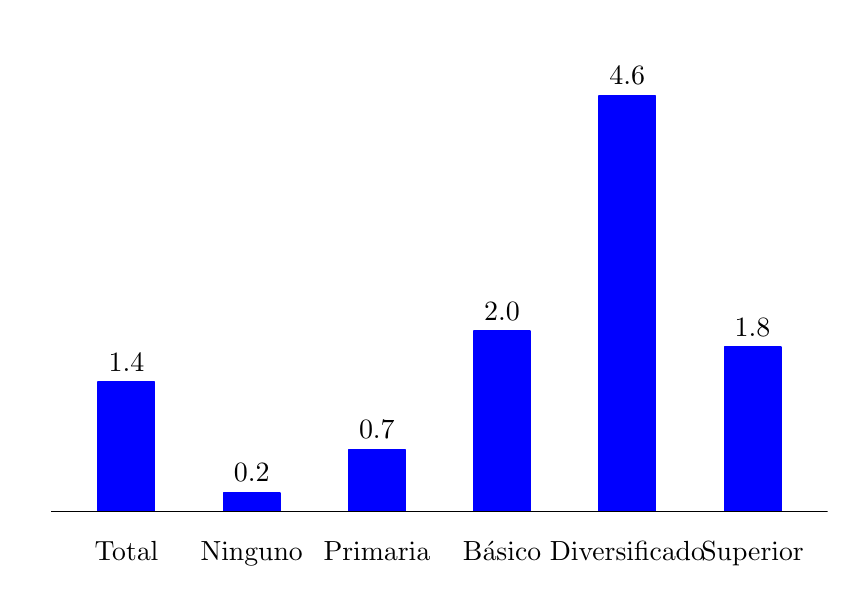
\begin{tikzpicture}[x=1pt,y=1pt]  % Created by tikzDevice version 0.9 on 2015-12-11 10:47:50
% !TEX encoding = UTF-8 Unicode
\definecolor{fillColor}{RGB}{255,255,255}
\path[use as bounding box,fill=fillColor,fill opacity=0.00] (0,0) rectangle (289.08,198.74);
\begin{scope}
\path[clip] (  0.00,  0.00) rectangle (289.08,198.74);

\path[] (  0.00,  0.00) rectangle (289.08,198.74);
\end{scope}
\begin{scope}
\path[clip] (  0.00,  0.00) rectangle (289.08,198.74);

\path[] (  8.54, 16.35) rectangle (289.08,181.67);

\path[] ( 35.69, 16.35) --
	( 35.69,181.67);

\path[] ( 80.93, 16.35) --
	( 80.93,181.67);

\path[] (126.18, 16.35) --
	(126.18,181.67);

\path[] (171.43, 16.35) --
	(171.43,181.67);

\path[] (216.68, 16.35) --
	(216.68,181.67);

\path[] (261.93, 16.35) --
	(261.93,181.67);
\definecolor{drawColor}{RGB}{0,0,255}
\definecolor{fillColor}{RGB}{0,0,255}

\path[draw=drawColor,line width= 0.6pt,line join=round,fill=fillColor] ( 25.50, 23.87) rectangle ( 45.87, 70.69);

\path[draw=drawColor,line width= 0.6pt,line join=round,fill=fillColor] ( 70.75, 23.87) rectangle ( 91.12, 30.62);

\path[draw=drawColor,line width= 0.6pt,line join=round,fill=fillColor] (116.00, 23.87) rectangle (136.36, 46.37);

\path[draw=drawColor,line width= 0.6pt,line join=round,fill=fillColor] (161.25, 23.87) rectangle (181.61, 89.07);

\path[draw=drawColor,line width= 0.6pt,line join=round,fill=fillColor] (206.50, 23.87) rectangle (226.86,174.16);

\path[draw=drawColor,line width= 0.6pt,line join=round,fill=fillColor] (251.75, 23.87) rectangle (272.11, 83.30);
\definecolor{drawColor}{RGB}{0,0,0}

\path[draw=drawColor,line width= 0.1pt,line join=round] (  8.54, 23.87) -- (289.08, 23.87);

\node[text=drawColor,anchor=base,inner sep=0pt, outer sep=0pt, scale=  1.01] at ( 35.69, 74.65) {1.4};

\node[text=drawColor,anchor=base,inner sep=0pt, outer sep=0pt, scale=  1.01] at ( 80.93, 34.58) {0.2};

\node[text=drawColor,anchor=base,inner sep=0pt, outer sep=0pt, scale=  1.01] at (126.18, 50.32) {0.7};

\node[text=drawColor,anchor=base,inner sep=0pt, outer sep=0pt, scale=  1.01] at (171.43, 93.02) {2.0};

\node[text=drawColor,anchor=base,inner sep=0pt, outer sep=0pt, scale=  1.01] at (216.68,178.11) {4.6};

\node[text=drawColor,anchor=base,inner sep=0pt, outer sep=0pt, scale=  1.01] at (261.93, 87.25) {1.8};

\path[] (  8.54, 16.35) rectangle (289.08,181.67);
\end{scope}
\begin{scope}
\path[clip] (  0.00,  0.00) rectangle (289.08,198.74);

\path[] (  8.54, 16.35) --
	(  8.54,181.67);
\end{scope}
\begin{scope}
\path[clip] (  0.00,  0.00) rectangle (289.08,198.74);

\path[] (  8.54, 16.35) --
	(289.08, 16.35);
\end{scope}
\begin{scope}
\path[clip] (  0.00,  0.00) rectangle (289.08,198.74);

\path[] ( 35.69, 12.08) --
	( 35.69, 16.35);

\path[] ( 80.93, 12.08) --
	( 80.93, 16.35);

\path[] (126.18, 12.08) --
	(126.18, 16.35);

\path[] (171.43, 12.08) --
	(171.43, 16.35);

\path[] (216.68, 12.08) --
	(216.68, 16.35);

\path[] (261.93, 12.08) --
	(261.93, 16.35);
\end{scope}
\begin{scope}
\path[clip] (  0.00,  0.00) rectangle (289.08,198.74);
\definecolor{drawColor}{RGB}{0,0,0}

\node[text=drawColor,anchor=base,inner sep=0pt, outer sep=0pt, scale=  1.00] at ( 35.69,  6.04) {Total};

\node[text=drawColor,anchor=base,inner sep=0pt, outer sep=0pt, scale=  1.00] at ( 80.93,  6.04) {Ninguno};

\node[text=drawColor,anchor=base,inner sep=0pt, outer sep=0pt, scale=  1.00] at (126.18,  6.04) {Primaria};

\node[text=drawColor,anchor=base,inner sep=0pt, outer sep=0pt, scale=  1.00] at (171.43,  6.04) {Básico};

\node[text=drawColor,anchor=base,inner sep=0pt, outer sep=0pt, scale=  1.00] at (216.68,  6.04) {Diversificado};

\node[text=drawColor,anchor=base,inner sep=0pt, outer sep=0pt, scale=  1.00] at (261.93,  6.04) {Superior};
\end{scope}
  \end{tikzpicture} }{Instituto Nacional de Estadística, con datos de ENEI II-2014}

%
%\cajita{Descoupados, escolaridad y sexo}{}{Proporción de la población desocupada, según nivel de escolaridad y sexo}{República de Guatemala, año 2014, en porcentaje}{\ \\[0mm]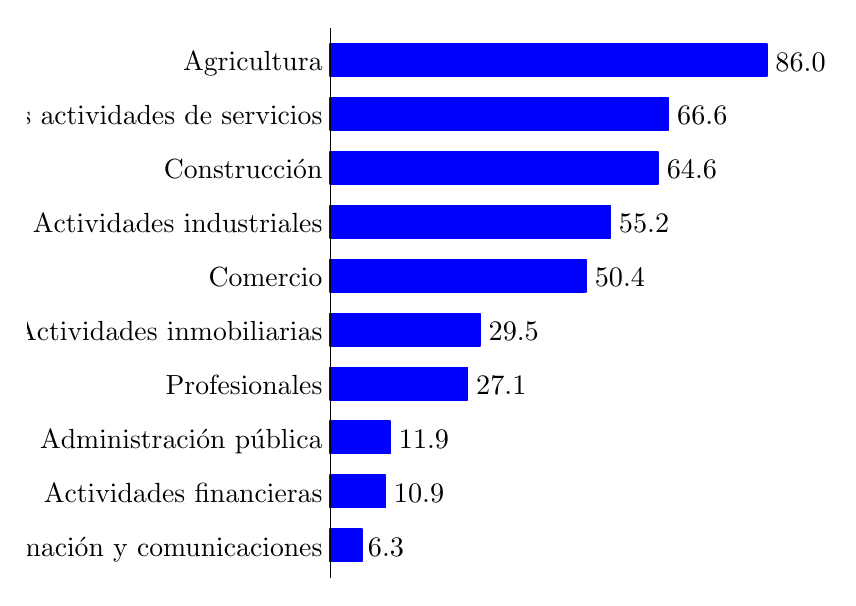
\begin{tikzpicture}[x=1pt,y=1pt]  % Created by tikzDevice version 0.9 on 2016-02-28 20:01:55
% !TEX encoding = UTF-8 Unicode
\definecolor{fillColor}{RGB}{255,255,255}
\path[use as bounding box,fill=fillColor,fill opacity=0.00] (0,0) rectangle (289.08,198.74);
\begin{scope}
\path[clip] (  0.00,  0.00) rectangle (289.08,198.74);

\path[] (  0.00,  0.00) rectangle (289.08,198.74);
\end{scope}
\begin{scope}
\path[clip] (  0.00,  0.00) rectangle (289.08,198.74);

\path[] (109.26,  0.00) rectangle (267.09,198.74);

\path[] (109.26, 11.69) --
	(267.09, 11.69);

\path[] (109.26, 31.18) --
	(267.09, 31.18);

\path[] (109.26, 50.66) --
	(267.09, 50.66);

\path[] (109.26, 70.14) --
	(267.09, 70.14);

\path[] (109.26, 89.63) --
	(267.09, 89.63);

\path[] (109.26,109.11) --
	(267.09,109.11);

\path[] (109.26,128.60) --
	(267.09,128.60);

\path[] (109.26,148.08) --
	(267.09,148.08);

\path[] (109.26,167.57) --
	(267.09,167.57);

\path[] (109.26,187.05) --
	(267.09,187.05);
\definecolor{drawColor}{RGB}{0,0,255}
\definecolor{fillColor}{RGB}{0,0,255}

\path[draw=drawColor,line width= 0.6pt,line join=round,fill=fillColor] (109.26,  5.85) rectangle (120.73, 17.54);

\path[draw=drawColor,line width= 0.6pt,line join=round,fill=fillColor] (109.26, 25.33) rectangle (129.25, 37.02);

\path[draw=drawColor,line width= 0.6pt,line join=round,fill=fillColor] (109.26, 44.81) rectangle (131.02, 56.51);

\path[draw=drawColor,line width= 0.6pt,line join=round,fill=fillColor] (109.26, 64.30) rectangle (158.94, 75.99);

\path[draw=drawColor,line width= 0.6pt,line join=round,fill=fillColor] (109.26, 83.78) rectangle (163.45, 95.47);

\path[draw=drawColor,line width= 0.6pt,line join=round,fill=fillColor] (109.26,103.27) rectangle (201.80,114.96);

\path[draw=drawColor,line width= 0.6pt,line join=round,fill=fillColor] (109.26,122.75) rectangle (210.55,134.44);

\path[draw=drawColor,line width= 0.6pt,line join=round,fill=fillColor] (109.26,142.24) rectangle (227.82,153.93);

\path[draw=drawColor,line width= 0.6pt,line join=round,fill=fillColor] (109.26,161.72) rectangle (231.57,173.41);

\path[draw=drawColor,line width= 0.6pt,line join=round,fill=fillColor] (109.26,181.21) rectangle (267.09,192.90);
\definecolor{drawColor}{RGB}{0,0,0}

\path[draw=drawColor,line width= 0.1pt,line join=round] (109.26,  0.00) -- (109.26,198.74);

\node[text=drawColor,anchor=base west,inner sep=0pt, outer sep=0pt, scale=  1.02] at (122.97,  7.72) {6.3};

\node[text=drawColor,anchor=base west,inner sep=0pt, outer sep=0pt, scale=  1.02] at (132.37, 27.20) {10.9};

\node[text=drawColor,anchor=base west,inner sep=0pt, outer sep=0pt, scale=  1.02] at (134.15, 46.69) {11.9};

\node[text=drawColor,anchor=base west,inner sep=0pt, outer sep=0pt, scale=  1.02] at (162.07, 66.17) {27.1};

\node[text=drawColor,anchor=base west,inner sep=0pt, outer sep=0pt, scale=  1.02] at (166.58, 85.66) {29.5};

\node[text=drawColor,anchor=base west,inner sep=0pt, outer sep=0pt, scale=  1.02] at (204.93,105.14) {50.4};

\node[text=drawColor,anchor=base west,inner sep=0pt, outer sep=0pt, scale=  1.02] at (213.67,124.63) {55.2};

\node[text=drawColor,anchor=base west,inner sep=0pt, outer sep=0pt, scale=  1.02] at (230.95,144.11) {64.6};

\node[text=drawColor,anchor=base west,inner sep=0pt, outer sep=0pt, scale=  1.02] at (234.70,163.60) {66.6};

\node[text=drawColor,anchor=base west,inner sep=0pt, outer sep=0pt, scale=  1.02] at (270.21,183.08) {86.0};

\path[] (109.26,  0.00) rectangle (267.09,198.74);
\end{scope}
\begin{scope}
\path[clip] (  0.00,  0.00) rectangle (289.08,198.74);

\path[] (109.26,  0.00) --
	(109.26,198.74);
\end{scope}
\begin{scope}
\path[clip] (  0.00,  0.00) rectangle (289.08,198.74);
\definecolor{drawColor}{RGB}{0,0,0}

\node[text=drawColor,anchor=base east,inner sep=0pt, outer sep=0pt, scale=  1.00] at (106.51,  7.78) {Información y comunicaciones};

\node[text=drawColor,anchor=base east,inner sep=0pt, outer sep=0pt, scale=  1.00] at (106.51, 27.27) {Actividades financieras };

\node[text=drawColor,anchor=base east,inner sep=0pt, outer sep=0pt, scale=  1.00] at (106.51, 46.75) {Administración pública };

\node[text=drawColor,anchor=base east,inner sep=0pt, outer sep=0pt, scale=  1.00] at (106.51, 66.24) {Profesionales};

\node[text=drawColor,anchor=base east,inner sep=0pt, outer sep=0pt, scale=  1.00] at (106.51, 85.72) {Actividades inmobiliarias};

\node[text=drawColor,anchor=base east,inner sep=0pt, outer sep=0pt, scale=  1.00] at (106.51,105.21) {Comercio };

\node[text=drawColor,anchor=base east,inner sep=0pt, outer sep=0pt, scale=  1.00] at (106.51,124.69) {Actividades  industriales};

\node[text=drawColor,anchor=base east,inner sep=0pt, outer sep=0pt, scale=  1.00] at (106.51,144.17) {Construcción};

\node[text=drawColor,anchor=base east,inner sep=0pt, outer sep=0pt, scale=  1.00] at (106.51,163.66) {Otras actividades de servicios};

\node[text=drawColor,anchor=base east,inner sep=0pt, outer sep=0pt, scale=  1.00] at (106.51,183.14) {Agricultura};
\end{scope}
\begin{scope}
\path[clip] (  0.00,  0.00) rectangle (289.08,198.74);

\path[] (106.51, 11.69) --
	(109.26, 11.69);

\path[] (106.51, 31.18) --
	(109.26, 31.18);

\path[] (106.51, 50.66) --
	(109.26, 50.66);

\path[] (106.51, 70.14) --
	(109.26, 70.14);

\path[] (106.51, 89.63) --
	(109.26, 89.63);

\path[] (106.51,109.11) --
	(109.26,109.11);

\path[] (106.51,128.60) --
	(109.26,128.60);

\path[] (106.51,148.08) --
	(109.26,148.08);

\path[] (106.51,167.57) --
	(109.26,167.57);

\path[] (106.51,187.05) --
	(109.26,187.05);
\end{scope}
  \end{tikzpicture} }{Instituto Nacional de Estadística, con datos de ENEI II-2014}
%

%\INEchaptercarta{Capacitación en el trabajo}{}
%



















